\documentclass[a4paper]{article}
\usepackage[spanish]{babel}
\usepackage[utf8]{inputenc}
\usepackage{charter}   % tipografia
\usepackage{graphicx}
\usepackage{courier}
%\usepackage{makeidx}
\usepackage{paralist} %itemize inline

%\usepackage{float}
\usepackage{amsmath, amsthm, amssymb}
%\usepackage{amsfonts}
%\usepackage{sectsty}
%\usepackage{charter}
%\usepackage{wrapfig}
%\usepackage{listings}
%\lstset{language=C}


\usepackage{fancyhdr}
\pagestyle{fancy}

%\renewcommand{\chaptermark}[1]{\markboth{#1}{}}
\renewcommand{\sectionmark}[1]{\markright{\thesection\ - #1}}

\fancyhf{}

\fancyhead[LO]{Sección \rightmark} % \thesection\ 
\fancyfoot[LO]{\small{Martín Fosco, Javier Minces, Cristian Chibana}}
\fancyfoot[RO]{\thepage}
\renewcommand{\headrulewidth}{0.5pt}
\renewcommand{\footrulewidth}{0.5pt}
\setlength{\hoffset}{-0.8in}
\setlength{\textwidth}{16cm}
%\setlength{\hoffset}{-1.1cm}
%\setlength{\textwidth}{16cm}
\setlength{\headsep}{0.5cm}
\setlength{\textheight}{25cm}
\setlength{\voffset}{-0.7in}
\setlength{\headwidth}{\textwidth}
\setlength{\headheight}{13.1pt}

\renewcommand{\baselinestretch}{1.1}  % line spacing
% \setcounter{secnumdepth}{2}
\usepackage{underscore}
\usepackage{caratula}
\usepackage{url}


\begin{document}


\thispagestyle{empty}
\materia{Métodos Numéricos}
\submateria{Segundo Cuatrimestre de 2014}
\titulo{Trabajo Práctico 2}
\subtitulo{Tirate un qu\'e, tirate un \emph{ranking}...}
\integrante{Fosco, Martin Esteban}{449/13}{mfosco65@gmail.com}
\integrante{Minces Müller, Javier Nicolás}{231/13}{javijavi1994@gmail.com}
\integrante{Chibana, Christian Ezequiel}{586/13}{christian.chiba93@gmail.com}

\maketitle
\newpage

\thispagestyle{empty}
\vfill
\begin{abstract}
En este trabajo se analizan tres métodos para crear un $ranking$ de páginas web: PageRank, HITS e In-Deg. Estos algoritmos utilizan matrices para modelar la Web mediante matrices y utilizan métodos numéricos, como el método de la potencia, para ordenar las páginas a partir de los links que las relacionan. %método, método, método
\end{abstract}

\thispagestyle{empty}
\vspace{3cm}
\tableofcontents
\newpage


%\normalsize
\newpage

\section{Introducci\'{o}n Te\'{o}rica}
\label{sec:intro}
%Contendrá una breve explicación de la base teórica que fundamenta los métodos involucrados en el trabajo, junto con los métodos mismos. No deben incluirse demostracionese de propiedades ni teoremas, ejemplos innecesarios, ni definiciones elementales (como por ejemplo la de matriz simétrica).

El problema a resolver es encontrar una manera confiable de definir en qué páginas es conveniente comprar espacios de propaganda para garantizar la mayor publicidad posible a un grupo de música.
El objetivo de este trabajo, por tanto, es resolver este problema analizado diferentes métodos que nos permitan definir un ranking de importancia de p\'{a}ginas web. \\

En un primer paso se debe acordar un m\'{e}todo de selecci\'{o}n de las p\'{a}ginas web sobre las cuales se trabaja, es decir que es necesario adquirir una subred de p\'{a}ginas relevantes al tema en cuesti\'{o}n

Se recurre en primer lugar a un buscador textual, pero este no asegura un resultado confiable en cuanto a la relevancia de las páginas recibidas. En el paper escrito por Kleinberg \footnote{Kleinberg - 1999 - \textit{Authoritative sources in a hyperlinked environment}} se sugiere un conjunto inicial de páginas $S_{\sigma}$ que cumple las siguientes condiciones:

\begin{itemize}

\item $S_{\sigma}$ es relativamente pequeña.
\item $S_{\sigma}$ contiene una gran cantidad de p\'{a}ginas relevantes.
\item $S_{\sigma}$ contiene muchas de las autoridades de m\'{a}s peso.

\end{itemize}

El autor propone una forma de ampliar este conjunto inicial para asegurar que se cumpla la tercera condición: buscar autoridades de gran peso a las que haya links en la subred obtenida del buscador e incluir \'{e}stas tambien en $S_{\sigma}$. 

Se construye luego un mapa de este conjunto de páginas en forma de grafo dirigido, observando los links entre ellas. Hasta este punto, el proceso escapa al objetivo del trabajo, que considera dado este mapa.\\ \\

Terminado este paso, se procede a construir la matriz de conectividad $W \in n \times n$, tal que $w_{ij}=1$ si existe un link de la página $j$ a la página $i$ y $w_{ij}=0$ en caso contrario. 

Usando esta matriz (con la misma notación), se pueden aplicar distintos m\'{e}todos para procesar y definir un cierto \textit{ranking} de las p\'{a}ginas.
Esta matriz es esparsa, porque incluso en redes de varios cientos de miles de páginas, en promedio cada una tiene 7 u 8 links salientes. \footnote{Kamvar}
Esto debe ser tenido en cuenta a la hora de guardar la matriz en memoria.

Los métodos a analizar son: \\


\textbf{PageRank}, el más conocido de los utilizados por Google. PageRank asigna un puntaje a cada página según el puntaje de las que apuntan a ella. De esta forma se evita que una página con muchos links de páginas sin valor obtenga un puntaje demasiado alto. Además, modifica W para tener en cuenta que un "navegante aleatorio" puede con una determinada probabilidad saltar a cualquier página de la web, algo que también hace si encuentra una página sin links salientes.

Esto se traduce como buscar un vector $x$ tal que $Wx=x$, es decir, encontrar el autovector para el autovalor 1. Si se sabe que 1 es el autovalor de mayor módulo, se puede encontrar su autovector con el método de las potencias.\\

\textbf{HITS} (Hyperlink-Induced Topic Search), este se basa en la existencia de páginas de gran valor como 'autoridad' y como "hub". En cada iteración, se actualiza el puntaje de cada página como autoridad a partir del puntaje hub de las páginas que la citan. Luego, se actualiza el puntaje como hub de cada página a partir del puntaje como autoridad de las páginas a las que apunta. Esto se puede reducir a una operación matricial.

\textbf{In-Deg}, El tercer método, el más intuitivo, se incluye principalmente como control. In-Deg consiste simplemente en contar los links que apuntan a cada página.\\

\newpage

\section{Desarrollo}
\label{sec:desarrollo}
%Deben explicarse los métodos numéricos que utilizaron y su aplicación al problema concreto involucrado en el trabajo práctico. Se deben mencionar los pasos que siguieron para implementar los algoritmos, las dificultades que fueron encontrando y la descripción de cómo las fueron resolviendo. Explicar también cómo fueron planteadas y realizadas las mediciones experimentales. Los ensayos fallidos, hipótesis y conjeturas equivocadas, experimentos y métodos malogrados deben figurar en esta sección, con una breve explicación de los motivos de estas fallas (en caso de ser conocidas).

%DEBERIAMOS PONER EN UNA PARTE DE METODOS MAL LOGRADOS, Q NO APROVECHABAMOS LA MATRIZ ESP PARA EL PRODUCTO NO?
%LO DE PASOS PARA IMPLEMENTAR LOS ALGORITMOS, TENDRIAMOS Q PONER Q PRIMERO HICIMOS EL MATRIZEsp Y LO DE CARGAR DATOS Snap (y dsp no me acuerdo la implementacion de page rank y hits al principio).
%Dificultades: Cargar de archivos con distintos renglones?, Leer los toronto (Problemas en el pageR seguro hubo, pero no me acuerdo.)
%Los ensayos fallidos, hipótesis y conjeturas equivocadas, experimentos y métodos malogrados??

\subsection{Criterio de almacenamiento}
Debimos primero encontrar una forma de almacenar los datos de los links entre p\'{a}ginas provistos (independientemente del formato en que fueron dados). Estos se guardan en la matriz $W$, ya mencionada.

Entre las 3 opciones sugeridas en el enunciado se opt\'{o} finalmente por el almacenamiento en forma de Compressed Sparse Column (CSC)\footnote{Una matriz esparsa que se recorre por columnas.} porque notamos que esto facilita aquellas operaciones que pueden ser necesarias para los algoritmos de mayor complejidad temporal (Pagerank y HITS) como:

\begin{itemize}

\item La suma de columnas (ya que se trata de sumar una secci\'{o}n de elementos contiguos del array en el que se guardan los valores de la matriz distintos de 0).

\item La divisi\'{o}n de una columna por una constante, debido a que al momento de definir en pagerank la probabilidad de salir de una p\'{a}gina a otra, debemos dividir las columnas de forma que sus elementos (las probabilidades de salir hacia alguna p\'{a}gina) sumen 1.

\item El producto de una matriz transpuesta por un vector, ya que puede recorrer una sección del vector de valores y multiplicarlos por una posición del vector. Para el producto de la matriz sin transponer el algoritmo es más complejo pero igual de eficiente: alcanza con recorrer los valores e ir acumulando en las distintas posiciones del vector resultado los valores parciales que se obtienen.

\end{itemize}

Además, tiene una eficiencia espacial \'{o}ptima para el almacenamiento de matrices que cuentan con muchos ceros (como es el caso de las matrices con las que trabajamos). M\'{a}s espec\'{i}ficamente : la memoria usada es $2 \times  O(m)+O(n)$.\footnote{$m$ es la cantidad de elementos diferentes de 0 y $n$ las filas de la matriz.} \\ 

En comparaci\'{o}n con las otras dos opciones de almacenamiento:

\begin{description}


\item[Dictionary of Keys] cuenta con s\'{o}lo la \'{u}ltima ventaja del CSC, que permite obviar a las posiciones en las que se guardan ceros, pero no es capaz de mejorar en ninguna manera la eficiencia de las operaciones matriciales, que se efect\'{u}an en los m\'{e}todos de ranking m\'{a}s complicados.

\item[Compressed Sparse Row (CSR)] cuenta con la \'{u}ltima ventaja del CSC tambi\'{e}n, pero no es capaz de operar con columnas de manera tan eficiente como el CSC.\\
Es necesario mencionar, sin embargo, que es una estructura m\'{a}s eficiente para realizar las operaciones que el \textit{In-Deg} requiere (por filas) por razones obvias, pero optamos por la \textit{Compressed Sparse Column} debido a que parece mejor optimizar las operaciones por columnas que intervienen en los algorítmos mas complejos (es posible modificar, sin embargo, las operaciones entre columnas para que se puedan realizar con una eficiencia análoga a las efectuadas por el CSC).
 
\end{description}

\newpage

\subsection{PageRank}

El algoritmo PageRank asigna un puntaje de importancia a cada página entre 0 y 1. Este no depende únicamente de la cantidad de links entrantes, sino que pondera cada link según el puntaje de la página al que pertenece. Sea $x$ el vector en $\mathbb{R}^n$ donde $x_j$ es el puntaje de la página $j$ y $n_j$ el $grado$ de $j$, es decir, la cantidad de links salientes, entonces se quiere ver que:
\begin{equation}
x_k = \sum_{j=1,w_{kj}=1}^{n} \frac{x_j}{n_j},~~~~k = 1,\dots,n.
\end{equation}

Supongamos que se tienen cuatro páginas para hacer el ranking (1, 2, 3, 4) y que están conectadas de esta forma:

$1 \rightarrow 2$

$1 \rightarrow 3$

$2 \rightarrow 3$

$3 \rightarrow 2$

$3 \rightarrow 4$

Entonces el problema se reduciría a buscar la solución a este sistema de ecuaciones:
\begin{center}
$\begin{bmatrix} 0&0&0&0\\\frac{1}{2}&0&\frac{1}{2}&0\\\frac{1}{2}&1&0&0\\0&0&\frac{1}{2}&0\end{bmatrix} \cdot \begin{bmatrix} x_1\\x_2\\x_3\\x_4 \end{bmatrix} = \begin{bmatrix} x_1\\x_2\\x_3\\x_4 \end{bmatrix}$
\end{center}
Llamamos $P$ a la matriz, que se construye dividiendo cada columna de $W$ por su suma. Se puede ver que la solución de este sistema de ecuaciónes es un vector $x$ tal que $Px=x$.

Se define un autovalor $\lambda$ de una matriz $A$ a un valor tal que $Ax=\lambda x$, y a $x$ como su autovector. En este caso, entonces, el problema se reduce a buscar un autovector para el autovalor 1. Dado que este autovector representa probabilidades, debe tener norma 1 igual a 1.

El método de la potencia permite encontrar el autovalor de mayor módulo de una matriz. Para poder aplicarlo en este caso, deben cumplirse las siguientes condiciones \footnote {Propuestas en \textit{Bryan, Leise - 2006 - The Linear Algebra behind Google $\ast$} y \textit{Kamvar, Haveliwala - 2003 - Extrapolation methods for accelerating PageRank computations}}:
\begin{itemize}
\item $P$ tiene un autovector asociado al autovalor 1
\item Los demás autovalores de la matriz cumplen $1 = \lambda_1 > |\lambda_2| \geq \dots \geq |\lambda_n|$ 
\item La dimensión del autoespacio asociado al autovalor $\lambda_1$ es 1: esto garantiza la unicidad del autovector de norma 1 igual a 1 asociado al autovalor 1.
\end{itemize}

Si la matriz $P$ es estocástica por columnas, se puede ver que se cumple las primeras dos condiciones:
Sea A una matriz en $\mathbb{R}^{n \times n}$ estocástica por columnas y sea $e$ un vector en $R^n$ tal que $e_i=1$ $\forall i$,
sabemos que $A$ y su transpuesta $A^T$ tienen los mismos autovalores. Como A es estocástica por columnas, se puede ver que $A^T e = e$, por lo que 1 es un autovalor de $A^T$ y, por tanto, de $A$. Además al estar dividida cada columna por su norma 1, la matriz es efectivamente estocástica por columnas, salvo que haya columnas cuya suma es 0. Esto se da en el caso de los llamados "dangling nodes", páginas sin links salientes. 

Se puede interpretar la navegación en la Web de un $navegante aleatorio$ como un proceso de Markov, a $P$ como su matriz de transición y a la componente $x_j$ del vector soluci\'on de norma 1 del sistema $Px = x$ como la proporci\'on del tiempo que el navegante pasa en la p\'agina $j$ Entonces, se puede suponer que al encontrarse en una página sin links salientes ($dangling node$), irá a cualquiera con probabilidad $1/n$. Se define entonces la matriz $P_1$, en la que se asigna 1/n, entonces, a cada fila de cada columna que representa un dangling node. En el ejemplo anterior:
\begin{center}
$P_1= \begin{bmatrix} 0&0&0&\frac{1}{6}\\\frac{1}{2}&0&\frac{1}{2}&\frac{1}{6}\\\frac{1}{2}&1&0&\frac{1}{6}\\0&0&\frac{1}{2}&\frac{1}{6} \end{bmatrix} $
\end{center}

Sin embargo, la última condición no se cumple necesariamente. Si se tienen dos subredes aisladas, entonces la dimensión del autoespacio será 2. Por ejemplo, sean las páginas (1,2,3,4), con los siguientes links: 

$1 \rightarrow 2$

$2 \rightarrow 1$

$3 \rightarrow 4$

$4 \rightarrow 3$

Su matriz de conectividad es:
\begin{center}
$W=\begin{bmatrix} 0&1&0&0\\1&0&0&0\\ 0&0&0&1\\0&0&1&0\end{bmatrix}$
\end{center}
Se puede ver que existen dos vectores diferentes de norma 1 tales que $Wx=x$, $x=\left( \frac{1}{2}, \frac{1}{2},0 ,0\right)$ y $x=\left(0,0,\frac{1}{2}, \frac{1}{2} \right)$ 

Para evitar esto, se agrega un parámetro $c>0$, donde $1-c$ representa la probabilidad de que un navegante aleatorio vaya a una página cualquiera. Se define entonces $P_2$ tal que
${P_2}_{ij} = c{P_1}_{ij} + \frac{1-c}{n}  \forall i$

$P_2$ cumple las tres condiciones, luego se puede buscar la solución de $P_2x=x$ con el método de la potencia. Sin embargo, no es esparsa; de hecho, no tiene ceros.

En el último ejemplo, con c=$4/5$:
\begin{center}
$W=\begin{bmatrix} \frac{1}{20}&\frac{17}{20}&\frac{1}{20}&\frac{1}{20}\\\frac{17}{20}&\frac{1}{20}&\frac{1}{20}&\frac{1}{20}\\ \frac{1}{20}&\frac{1}{20}&\frac{1}{20}&\frac{17}{20}\\\frac{1}{20}&\frac{1}{20}&\frac{17}{20}&\frac{1}{20}\end{bmatrix}$
\end{center}

Y el PageRank resultante sería: \\

\indent 1: 0,25 \\
\indent 2: 0,25 \\
\indent 3: 0,25 \\
\indent 4: 0,25 \\

\subsubsection{M\'{e}todo de la Potencia}

Este método permite encontrar al autovalor de mayor módulo de una matriz.

Sea $A \in \mathbb{R}^{n \times n}$, $\lambda_1 ... \lambda_n$ sus autovalores tales que $|\lambda_1|>|\lambda_2| \geq ... \geq |\lambda_n|$, $v_1$ ... $v_n$ una base de autovectores
%Si quieren dar vueltas, se puede demostrar que esto existe
y $x$ un vector cualquiera. $x$ se puede escribir como combinación lineal de los autovectores de $A$:
\begin{eqnarray*}
x & = &\sum_{j=1}^{n} \alpha_j v_j\\
Ax & = &\sum_{j=1}^{n} \alpha_j Av_j
\end{eqnarray*}

Como $v_j$ es autovector de $A$, entonces:
\begin{eqnarray*}
Ax&=&\sum_{j=1}^{n} \alpha_j \lambda_j v_j\\
A^2x&=&\sum_{j=1}^{n} \alpha_j \lambda_j Av_j\\
A^2x&=&\sum_{j=1}^{n} \alpha_j \lambda^2_j v_j
\end{eqnarray*}

\begin{eqnarray*}
&.&\\
&.&\\
&.&\\
A^kx&=&\lambda_1^k \cdot (\sum_{j=1}^{n} \frac {\lambda_j}{\lambda_1}^k v_j)\\
A^kx&=&\lambda_1^k \cdot (\alpha_1 v_1 \sum_{j=2}^{n} \frac {\lambda_j}{\lambda_1}^k v_j)\\
\frac{||A^kx||}{||A^{k-1x||}}&=&\frac{||\lambda_1^k \cdot (\alpha_1 v_1 \sum_{j=2}^{n} \frac {\lambda_j}{\lambda_1}^k v_j)||}{||\lambda_1^{k-1} \cdot (\alpha_1 v_1 \sum_{j=2}^{n} \frac {\lambda_j}{\lambda_1}^{k-1} v_j)||}\\
\end{eqnarray*}
cuando $k \rightarrow \infty$, $\frac{\lambda_j}{\lambda_1} \rightarrow 0$ porque $\lambda_1>\lambda_j$ $\forall j$, luego 
\begin{eqnarray*}
\frac{||A^kx||}{||A^{k-1}x||} \rightarrow \frac{||\lambda_1^k \cdot (\alpha_1 v_1) ||}{||\lambda_1^{k-1} \cdot (\alpha_1 v_1)||} = \lambda_1
\end{eqnarray*}

$A^kx=((...((AA)A)...A)A)x=A(A(A(...(A(Ax)))$\\
%Faltaria explicar porq A a la k por x te da el aoutovector asociado al autovalor 1
Es decir que se puede implementar un algoritmo que calcule $Ax$ y asigne el resultado a $x$, siendo este el autovector buscado.

Para el contexto particular del PageRank, utilizamos el algoritmo 1 propuesto por Kamvar\footnote{Kamvar, Haveliwala - 2003 - Extrapolation methods for accelerating PageRank computations}, que permite calcular $P_2 x$ a partir de $Px$. Esto permite ahorrar tiempo y memoria, ya que $P$ es una matriz esparsa. El algoritmo consiste de tres pasos:
\begin{eqnarray*}
y&=&c(Px)\\
w&=&||x||_1-||y||_1\\
y&=&wv\\
\end{eqnarray*}

Donde $v$ es un vector en $ \textbf{R}^n$ tal que $v_i=1/n \forall i$

Es decir, $y_i=c(Px)_i+(1-c||Px||_1)/n$ \\
%||Px||&=&\sum_j (Px_j)\\
%(Px_j)&=&\sum_i p_{ji} x_i

%||Px||=suma_j (Px_j)

%||Px||=suma_j (sum_i p_{ji} x_i)

%||Px||=suma_i x_i·(sum_j p_{ji})

%sum_j p_{ji}=0:

%||Px||=0 => (Px)_i=0 \forall i

%$y_i=1/n$ \\

%sum_j p_{ji}>0:

\subsection{Hits}

La idea detr\'as de este m\'etodo es, como se ha explicado brevemente antes, realizar un an\'{a}lisis de la red y sus p\'aginas vi\'endolas como hubs y autoridades, nociones que son definidas por las relaciones (links) que tienen con el resto de la red.\\

Dada una b\'{u}squeda, el objetivo es retornar un subconjunto de páginas relevantes.
Se asigna entonces sobre las p\'aginas el rol de $autoridad$ en el tema que se busca. Su valor como $autoridad$ est\'a definido por el valor de $hub$ de las p\'{a}ginas que apuntan a ella mientras que el valor o peso de $hub$ est\'a definido, a su vez, por el valor de $autoridad$ de las p\'{a}ginas a las que apunta.\\

Recordemos que los links están almacenados en la matriz de conectividad $W^t$ donde $w^t_{ij} = 1$ si existe un link de la p\'agina $j$ a la p\'agina $i$,  $w^t_{ij} = 0$ en caso contrario. Para cada p\'agina $i \in Web$ se define como peso de autoridad $x_i$ y como peso de hub $y_i$.
A partir de esto, podemos definir los vectores $x,y \in \mathbb{R}^n$ como los vectores de pesos de autoridad y hubs, y se puede suponer que se encuentran normalizados.
Evidentemente, se desprende de esto que las p\'{a}ginas con mayores $x_i$ o $y_i$ son consideradas las mejores $autoridades$ o $hubs$.

Se puede expresar la transferencia de pesos de hubs y autoridad, respectivamente, de la siguiente manera:

\begin{description}

\item[Peso de Autoridad] $x_j = \sum_{i} y_i$

\item[Peso de Hub] $y_i = \sum_{j} x_j$

\end{description}

Consecuentemente, si expresamos con operaciones matriciales los vectores de hub y autoridad:
\begin{eqnarray*}
x &=& Wy \\
y &=& W^tx
\end{eqnarray*}

Se aplica luego el paso de normalizaci\'{o}n $y \leftarrow \frac{y}{||y||}$ y se vuelve a comenzar hasta llegar a la convergencia.
Para la primera iteraci\'{o}n es posible empezar con un $y_0$ inicial cualquiera, y el m\'{e}todo converger\'{a} si se cumplen las siguientes condiciones:

\begin{itemize}
\item $W$ tiene un autovalor $\lambda_1$ tal que $|\lambda_1| > |\lambda_2| \geq \dots \geq |\lambda_n|$ 
\item $y_0$ no es ortogonal al autovector asociado a $\lambda_1$
\end{itemize}

% Justificación: (creo que esta es la parte opcional).

%One easily verifies that the I and O operations can be written $x \leftarrow A^T y$ and $y \leftarrow Ax$, respectively. Thus, $x_k$ is the unit vector in the direction of $(A^T A)^{k-1}z$, and $y_k$ is the unit vector in the direction of $(AA^T)^kz$.

%Now, a standard result of linear algebra states that if $M$ is a symmetric $n \times n$ matrix, and $v$ is a vector not orthogonal to the principal eigenvector $\lambda 1 (M)$, then the unit vector in the direction of $M^k v$ converges to $\lambda_1 (M)$ as $k$ increases without bound.

%Also (as a corollary), if $M$ has only nonnegative entries, then the principal eigenvector of $M$ has only nonnegative entries.

%Consequently, $z$ is not orthogonal to $\lambda_1 (A A^T)$, and hence the sequence $\{y^k\}$ converges to a limit $y^*$. Similarly, one can show that if $\lambda_1 ( A^T A) \neq 0$ (as dictated by Assumption ()), then $A^T z$ is not orthogonal to $\lambda 1 ( A^T A)$. It follows that the sequence $\{x^k\}$ converges to a limit $x^*$.

\subsection{In-Deg}

Este m\'etodo es considerablemente m\'{a}s simple y sigue una idea m\'{a}s intuitiva de ranking de p\'aginas sin llegar a entrar en complejizaciones para tener en cuenta distintos casos, lo que consideramos que lleva a unos resultados menos fiables. Esto se debería notar especialmente cuando son contrastados con aquellos que obtenemos de analizar redes con m\'etodos que dan m\'as peso a detalles que potencialmente cambiarían los resultados (por ejemplo: una página apuntada por pocas páginas de gran valor caería muy por debajo en el ranking, mientras que probablemente PageRank y HITS le asignarían una posición más alta).

La idea b\'asica es definir el valor de un p\'agina seg\'un la cantidad de p\'aginas que la apuntan.

En otras palabras: el método consiste en sumar los links a cada página y, teniendo en cuenta que ya contamos con la matriz $W$, este método se reduce a sumar la fila correspondiente a cada página y obtener as\'i un vector que nos muestra el valor de cada una (la i\'esima posición corresponde a la iésima página, según su posición asignada en la matriz $W$). 


\subsection{Experimentos realizados}
Para los dos primeros métodos, se realizaron experimentos para ver la convergencia de la diferencia en cada iteración de la norma del autovector buscado. En PageRank, se utilizo la norma 1 del autovector $x$. En el caso de HITS, se analizó los vectores $x$ e $y$ tomando norma 2.
Luego, se comparó el tiempo de ejecución de cada uno utilizando la librería time.h de C++. No se tomó en cuenta el tiempo que toma cargar la matriz. Como una iteración de HITS hace dos productos de una matriz por un vector, mientras que PageRank hace uno, y que esta operación es la que domina el costo temporal de la ejecución, se esperaba que el tiempo de ejecución de HITS fuera alrededor del doble del de PageRank, independientemente del valor de $c$ usado. Este influye en el tiempo de ejecución\footnote{Kamvar, Haveliwala - 2003 - Extrapolation methods for accelerating PageRank computations} pero no esperábamos que modificara sustancialmente esta relación.

Dado que indexamos la matriz desde 1, reemplazamos cada página numerada como 0 por $n+1$ para poder realizar los tests.

Las instancias de test usadas fueron las siguientes:\\ \\
\begin{tabular}{c|r |r |r}
$\sigma$ & nodos & links & $\frac{link}{nodo}$\\
\hline
Movie & 5.757 & 24.451 & 4,24\\
\hline
Censorship & 2.947 & 9.555 & 3,24\\
\hline
Genetic & 3.468 & 12.689 & 3,65 \\
\hline
NotreDame & 325.729 & 1.497.134 & 4,59 \\
\hline
Stanford & 281.903 & 2.312.497 & 8,20 \\
\end{tabular}

Los valores de $c$ usados para el pageRank fueron los siguientes:
\begin{itemize}
\item 0.5
\item 0.7
\item 0.85
\item 0.95
\end{itemize}
Mientras que la tolerancia para asumir convergencia la fijamos en $10^{-4}$

A continuación se experimentó con una muestra de links entre varias páginas obtenida mediante el script provisto por la cátedra. De esta forma esperábamos analizar los resultados obtenidos en función de qué páginas se esperaban con mayor ranking.
%Experimentos:
%Ver la covergencia de la norma 1 de Pagerank
%Ver la convergencia de la norma ¿2? de HITS
%Comparar tiempos
%Comparar calidades

\newpage
\section{Resultados}
\label{sec:res}
%Deben incluir los resultados de los experimentos, utilizando el formato más adecuados para su presentación. Deberán especificar claramente a qué experiencia corresponde cada resultado. No se incluirán aquí corridas de máquina.
\subsection{Convergencia de Norma Manhattan de Pagerank}

Estos son los resultados obtenidos de convergencia de la norma para los distintos tests.

En los gráficos de PageRank se compara la evolución de $||x^k-x^{k-1}||_1$ para distintos valores de $c$.\\

\begin{figure}[htbp]
\centering
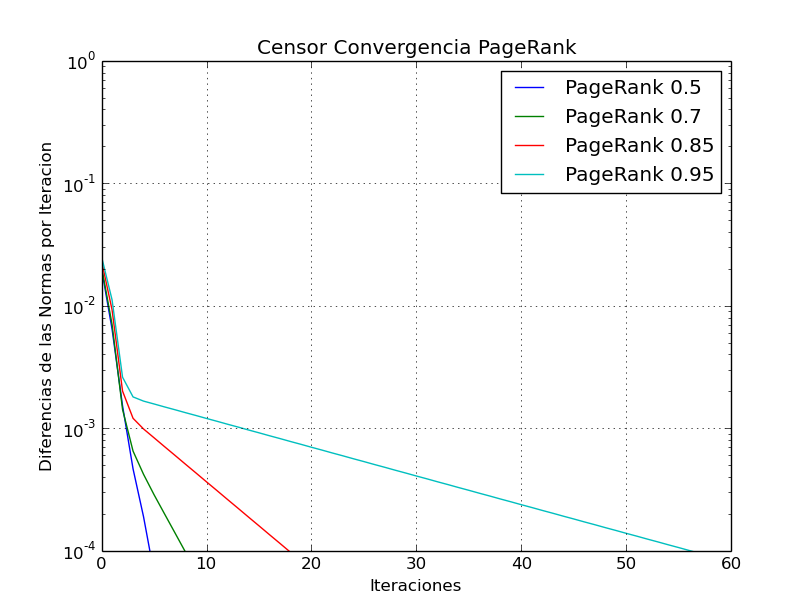
\includegraphics[scale=0.25]{img/Normas-Page-Censor.png} 
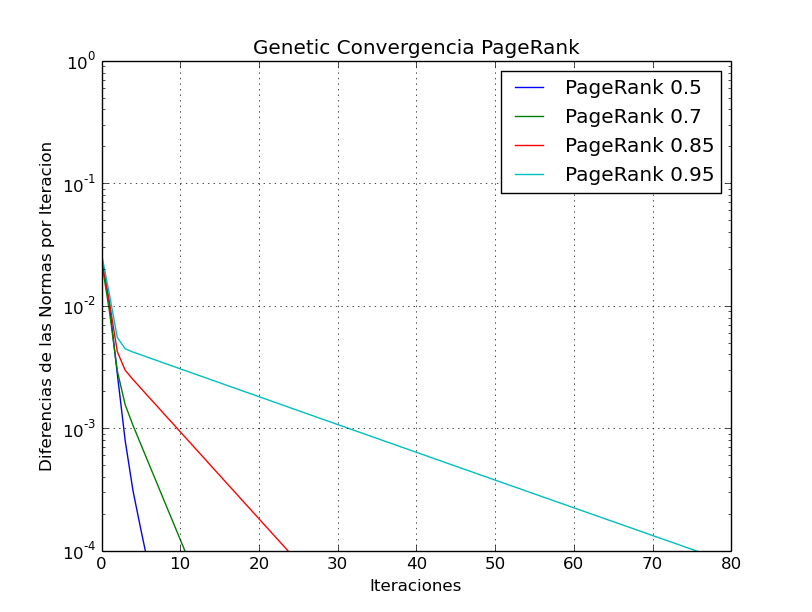
\includegraphics[scale=0.25]{img/Normas-Page-Genetic.png} 
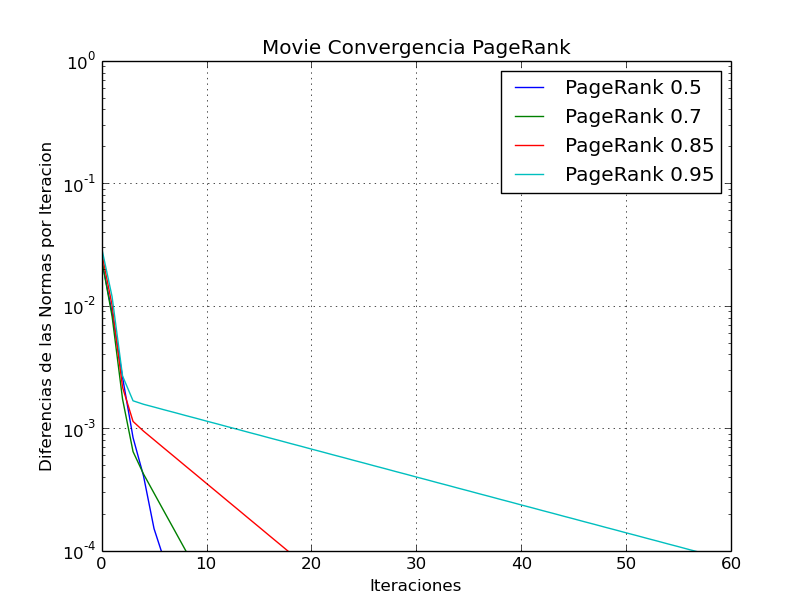
\includegraphics[scale=0.25]{img/Normas-Page-Movie.png}

\caption{Normas (PageRank): escala logarítmica}
\end{figure}

\begin{center}
\begin{tabular}{r|c|c|c}
&  \textbf{Censorship} & \textbf{Genetic} & \textbf{Movies} \\ 
\hline
C & Iteración de Llegada & Iteración de Llegada & Iteración de Llegada\\
\hline
0.5 & 6 & 7 & 7\\
\hline
0.7 & 9 & 12 & 10\\
\hline
0.85 & 19 & 25 & 19\\
\hline
0.95 & 58 & 77 & 58
\end{tabular}
\end{center}


\begin{figure}[htbp]
\centering
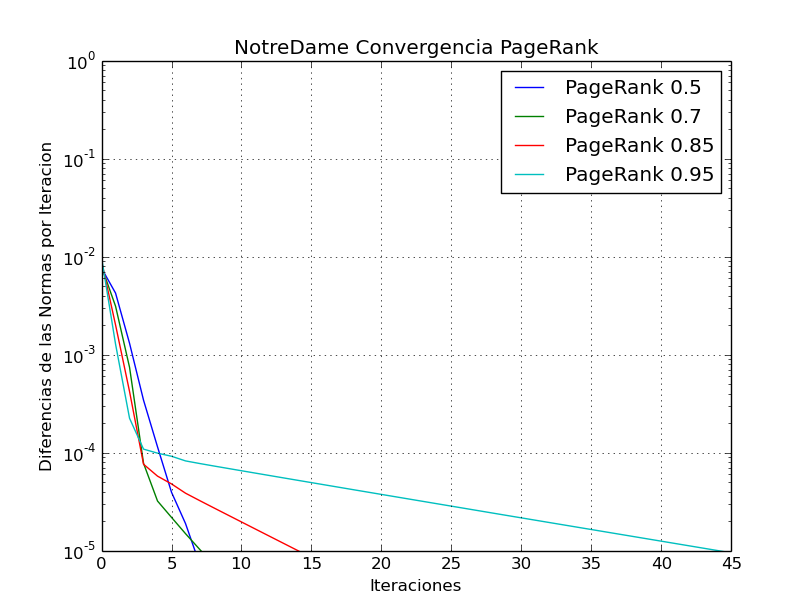
\includegraphics[scale=0.35]{img/Normas-Page-Notre.png}
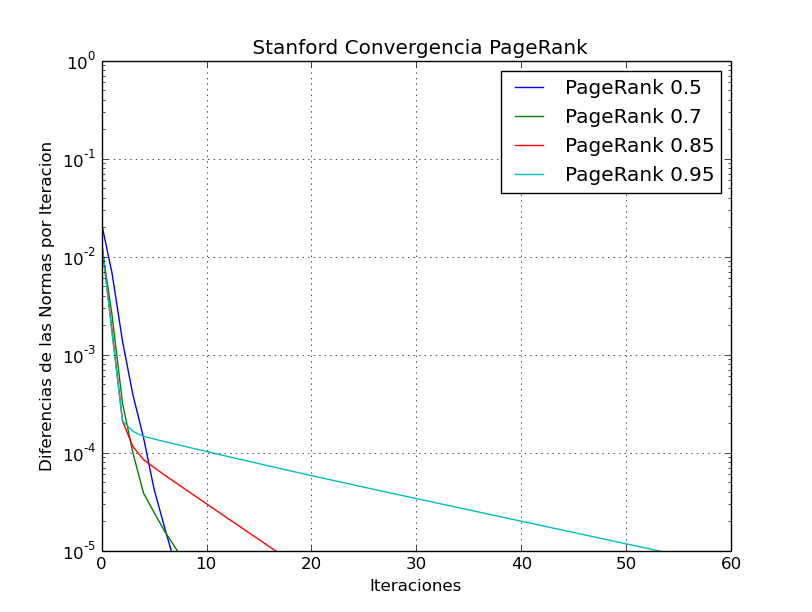
\includegraphics[scale=0.35]{img/Norma-Page-Stanford.png}
\caption{Normas (PageRank): escala logarítmica}
\end{figure}

\begin{center}
\begin{tabular}{r|c|c}
 & \textbf{Notredame} & \textbf{Stanford}\\
\hline
C & Iteración de Llegada & Iteración de Llegada \\
\hline
0.5 & 8 & 8\\
 \hline
0.7 & 9 & 9\\
\hline
0.85 & 16 & 18\\
\hline
0.95 & 46 & 55
\end{tabular}
\end{center}

%\caption{Normas (PageRank): escala logarítmica}
%\label{fig:graficos_cropflip}

\newpage

En los gráficos de HITS se compara la evolución de $||x^{(k)}-x_{(k-1)}||_2$ con la de $||y^{(k)}-y^{(k-1)}||_2$.\\
\begin{figure}[htbp]
\centering
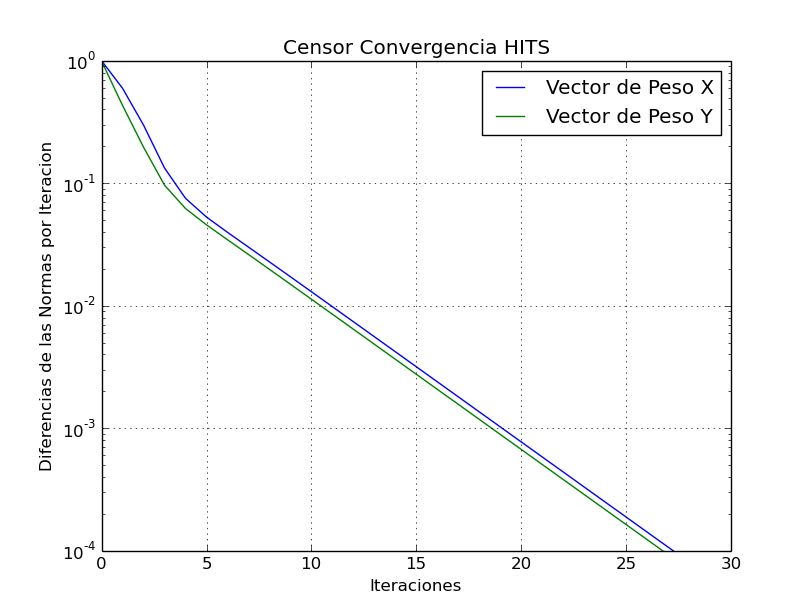
\includegraphics[scale=0.25]{img/Normas-HITS-Censor.png}
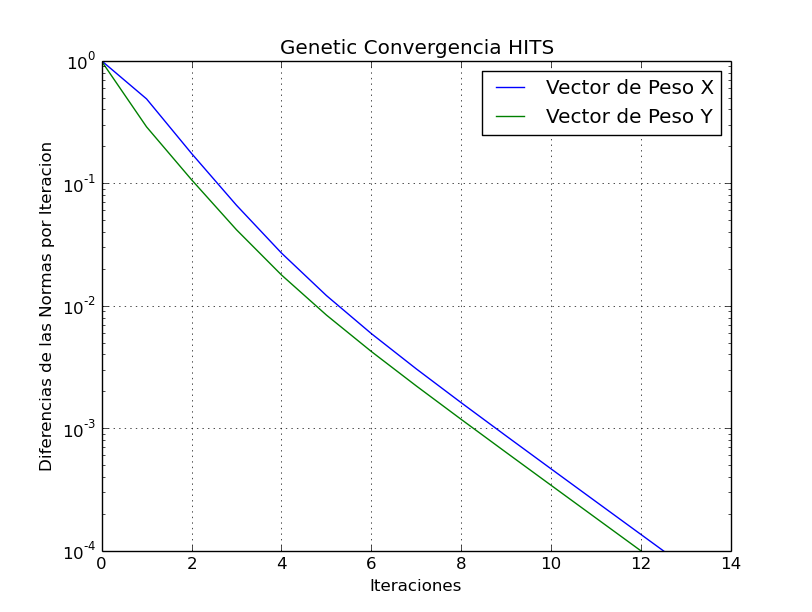
\includegraphics[scale=0.25]{img/Normas-HITS-Genetic.png} 
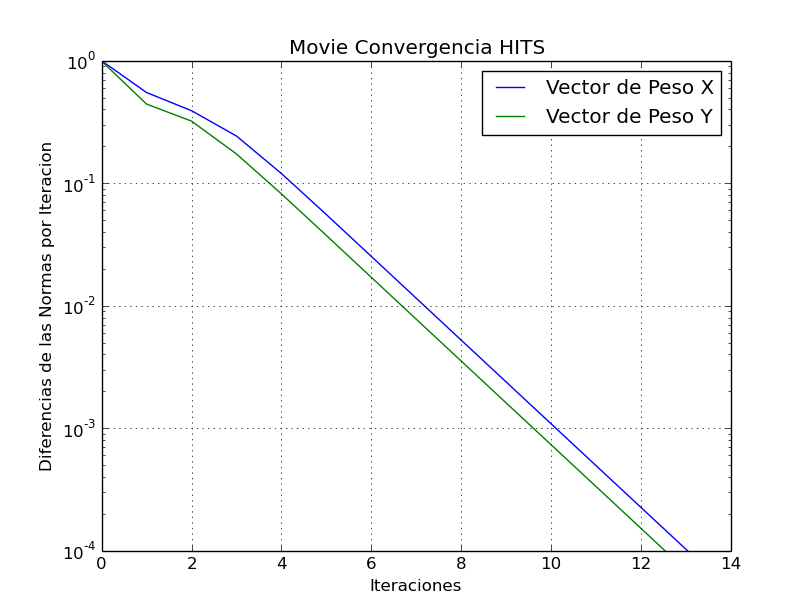
\includegraphics[scale=0.25]{img/Normas-HITS-Movie.png}

\caption{Normas (HITS): escala logarítmica}
\end{figure}

\begin{center}

\begin{tabular}{r|c|c|c}
&  \textbf{Censorship} & \textbf{Genetic} & \textbf{Movies} \\ 
\hline
 Iteración de Llegada & 29 & 14 & 15\\

\end{tabular}


\end{center}


\begin{figure}[htbp]
\centering
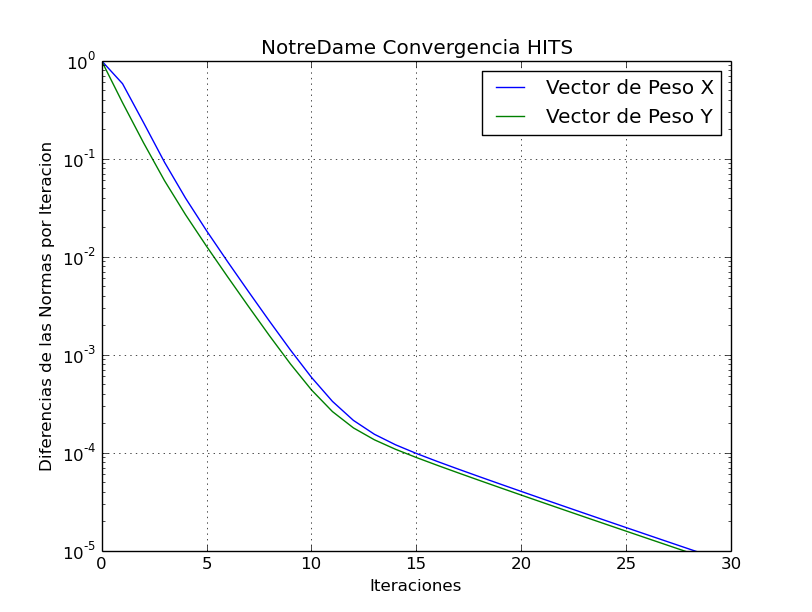
\includegraphics[scale=0.385]{img/Normas-HITS-Notre.png}
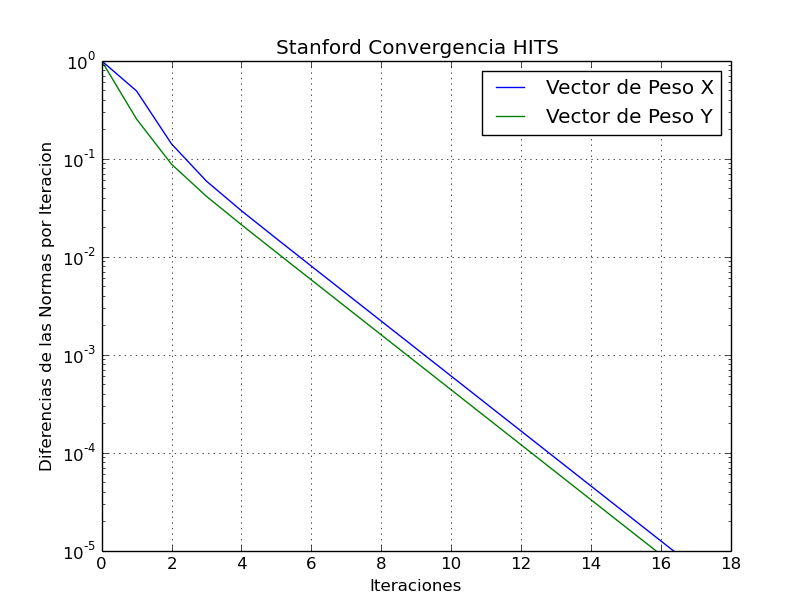
\includegraphics[scale=0.385]{img/Norma-HITS-Stanford.png}
\caption{Normas(HITS): escala logarítmica}
\label{fig:graficos_cropflip}
\end{figure}

\begin{center}

\begin{tabular}{r|c|c}
&  \textbf{NotreDame} & \textbf{Stanford}\\ 
\hline
 Iteración de Llegada & 30 & 18\\
\end{tabular}

\end{center}

Estos son los resultados de tiempo de cómputo obtenidos, en ciclos de clock:

\begin{figure}[htbp]
\centering
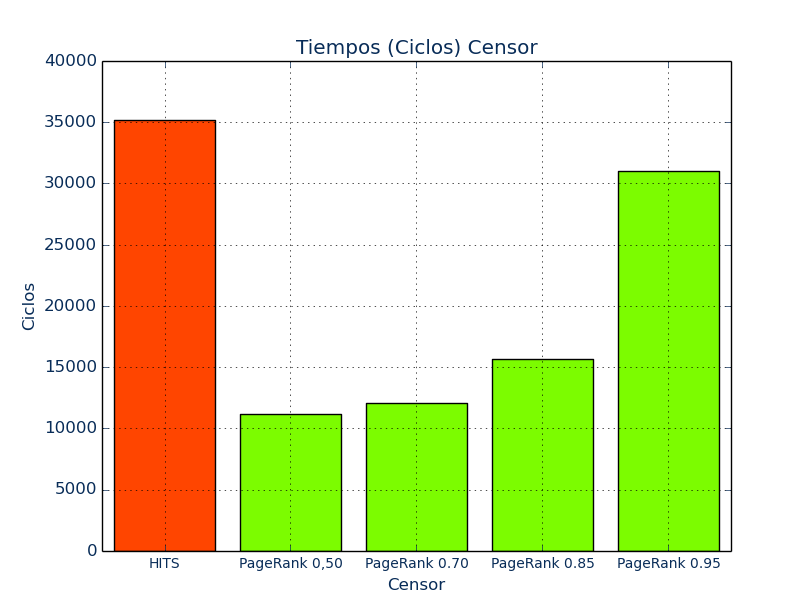
\includegraphics[scale=0.25]{img/Tiempos-Censor.png}
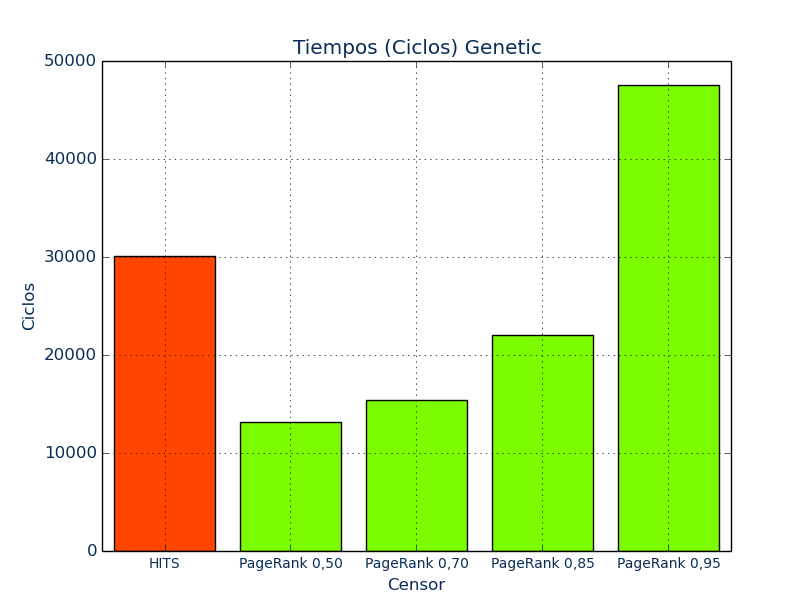
\includegraphics[scale=0.25]{img/Tiempos-Genetic.png}
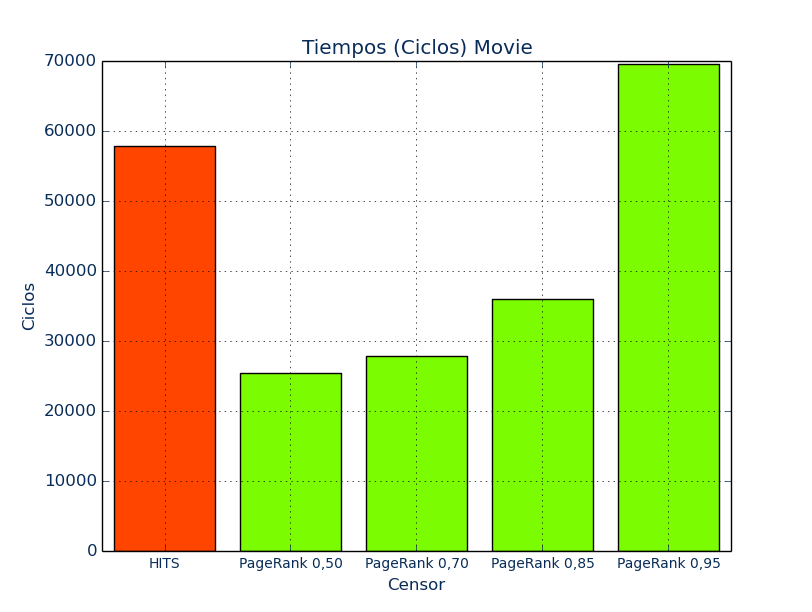
\includegraphics[scale=0.25]{img/Tiempos-Movie.png}
\caption{Tiempo de cómputo}
\end{figure}

\begin{figure}[htbp]
\centering
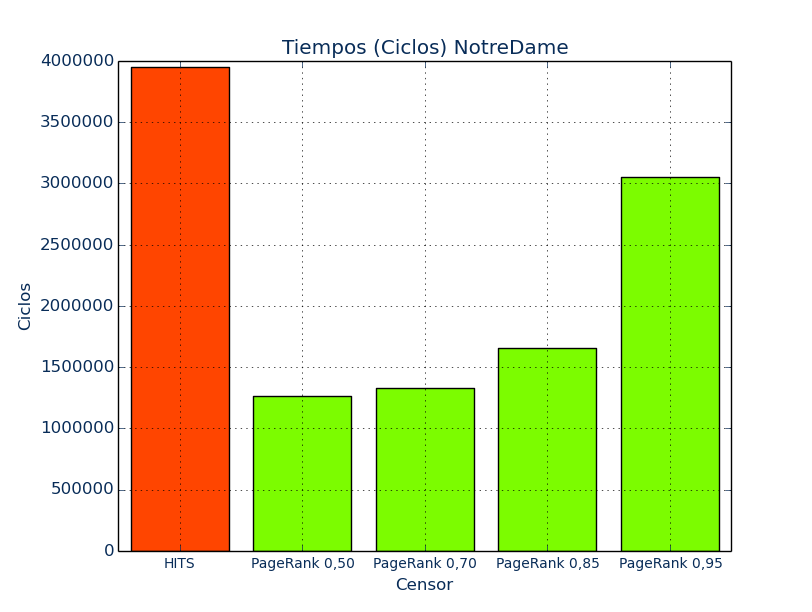
\includegraphics[scale=0.385]{img/Tiempos-Notre.png}
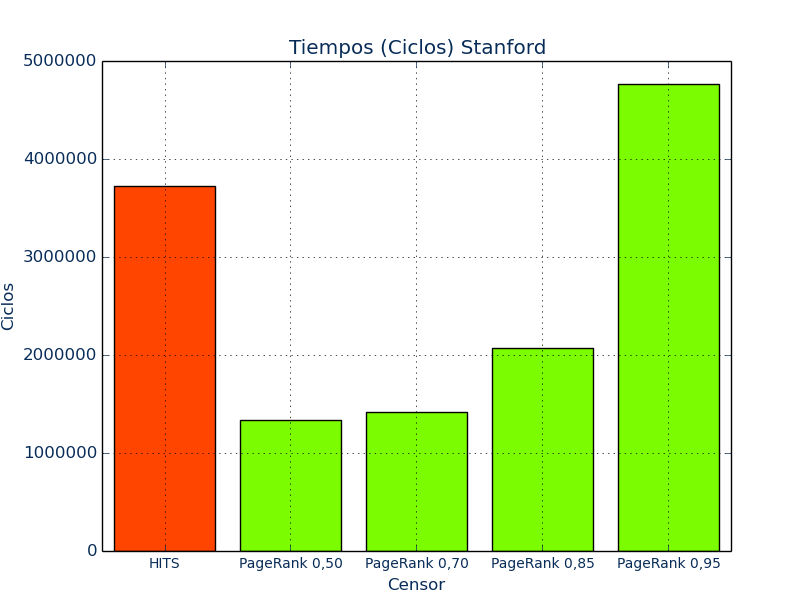
\includegraphics[scale=0.385]{img/Tiempo-Stanford.png}
\caption{Tiempo de cómputo}
\end{figure}

\newpage
\begin{center}
\begin{tabular}{l|c|c|c|c|c}
\hline
& Movie & Censorship & Genetic & NotreDame & Stanford\\
\hline
Ciclos por Iteración PageRank & 1896.1 & 822 & 882.2 & 103619.1 & 115099.8 \\
\hline
Ciclos por Iteración HITS & 3857.8 & 1213.4 & 2149.5 & 131540.1 & 206502.1
\end{tabular}
\end{center}

\subsection{Puntajes obtenidos}

\begin{figure}[htbp]
\centering
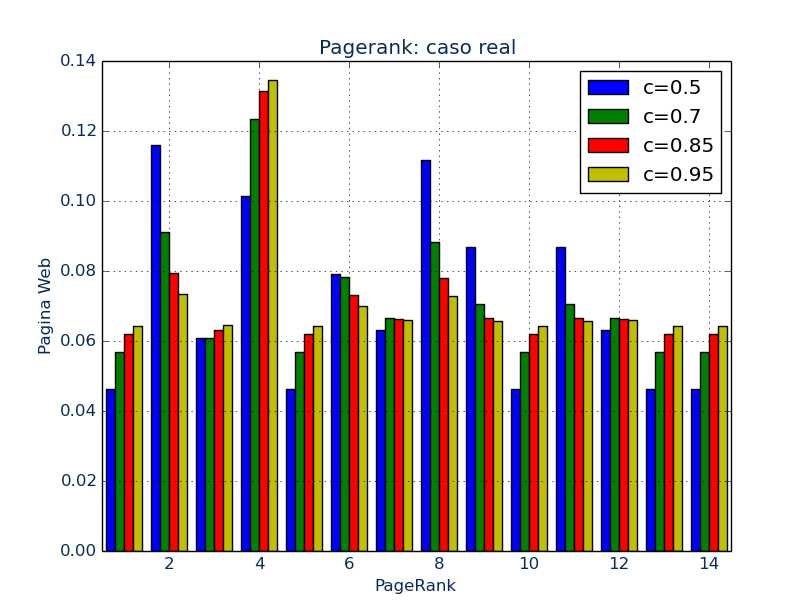
\includegraphics[scale=0.25]{img/casorealPage.png}
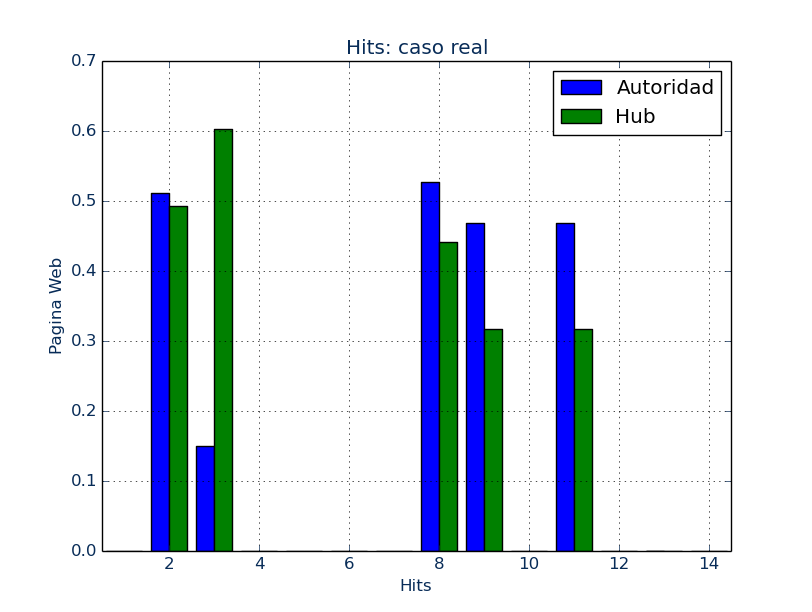
\includegraphics[scale=0.25]{img/casorealHits.png}
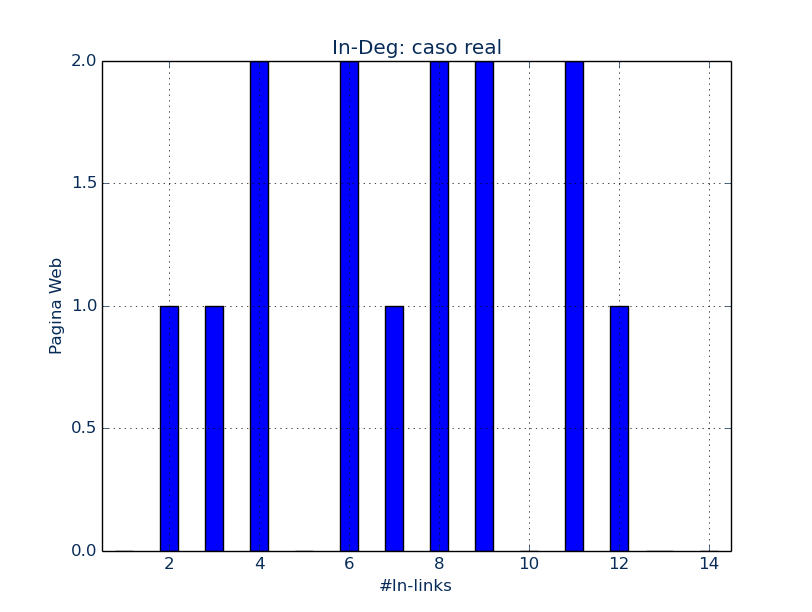
\includegraphics[scale=0.25]{img/casorealIn-Deg.png}
\caption{Puntajes obtenidos con los distintos métodos por distintas páginas}
\end{figure}

\begin{tabular}{r|l}
1 & www.google.com\\
2 & www.clarin.com\\
3 & www.clarin.com/deportes\\
4 & www.lanacion.com.ar\\
5 & www.infobae.com\\
6 & canchallena.lanacion.com.ar\\
7 & www.rollingstone.com.ar\\
8 & www.ole.com.ar \\
9 & www.clasificados.clarin.com\\
10 & www.mamapuntocero.com.ar\\
11 & www.ciudad.com.ar\\
12 & www.zonaprop.com.ar\\
13 & www.pagina12.com.ar\\
14 & www.yahoo.com\\
\end{tabular}

\subsection{Redes pequeñas}
Consideramos los siguientes casos:
\begin{itemize}
\item Una red en la que una página apunta a todas
\item Una red en la que todas las páginas apuntan a una
\item Una red en la que casi todas las páginas se apuntan entre sí
\item Una red con muy pocos links
\end{itemize}
Para observar el comportamiento de PageRank y HITS. Obtuvimos estos resultados:

\begin{figure}[htbp]
\centering
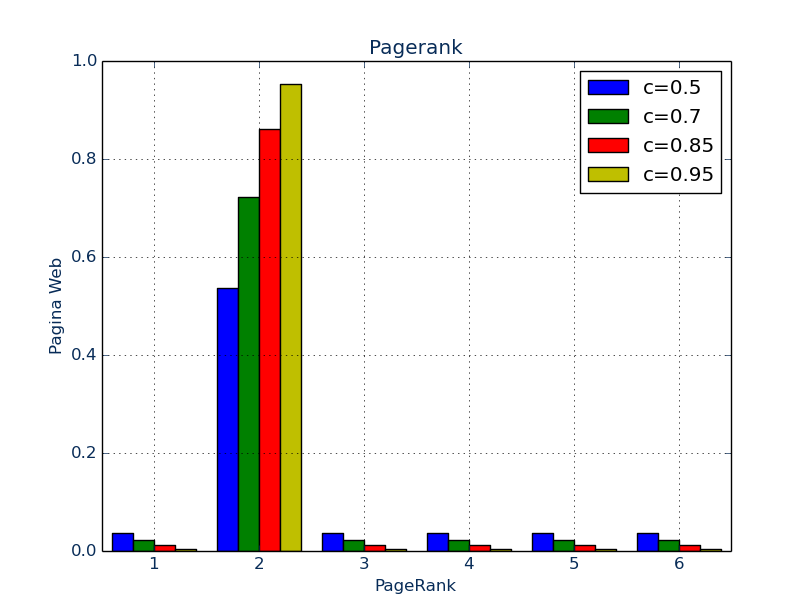
\includegraphics[scale=0.385]{img/todosal2.png}
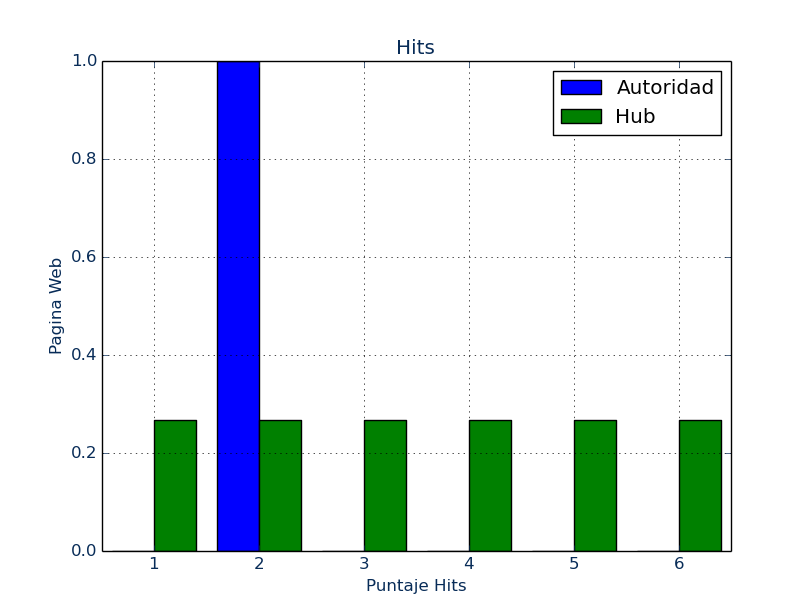
\includegraphics[scale=0.385]{img/todosal2out.png}
\caption{Puntajes obtenidos para una red en la que todas las páginas apuntan a la nº 2}
\end{figure}

\begin{figure}[htbp]
\centering
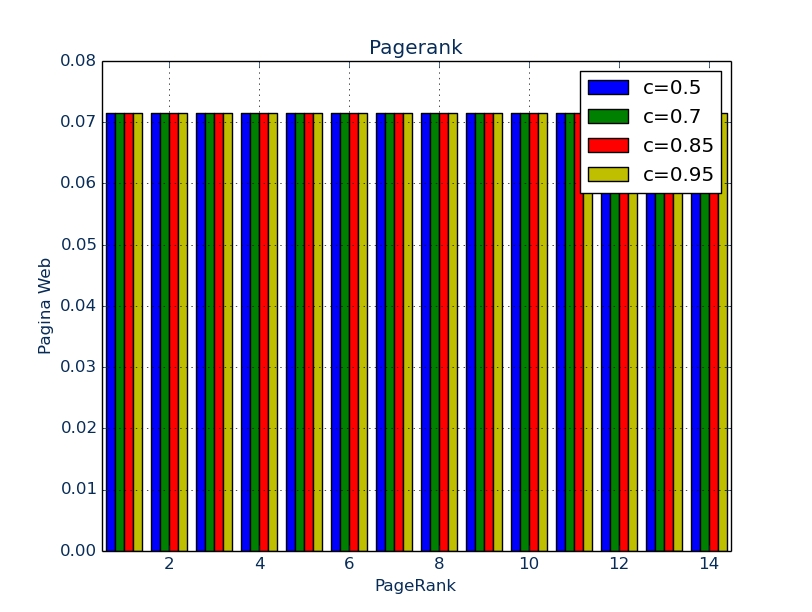
\includegraphics[scale=0.385]{img/eldosatodos.png}
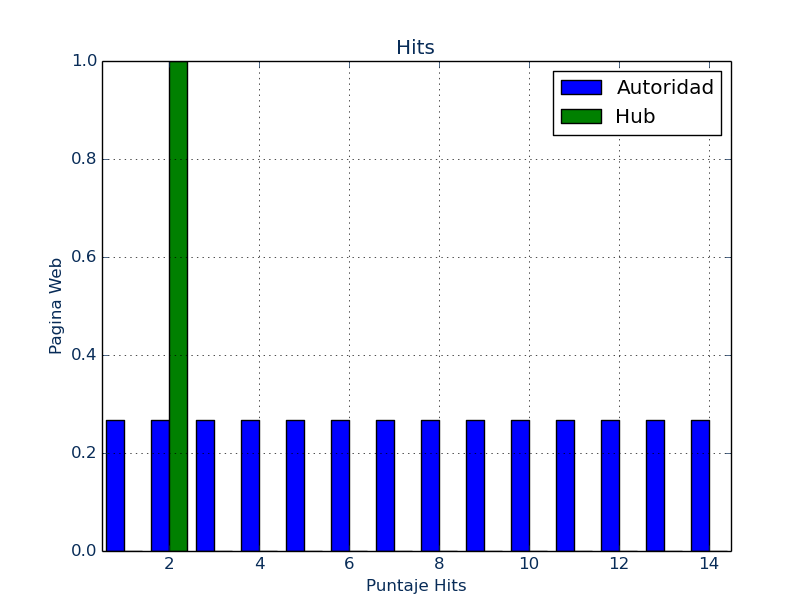
\includegraphics[scale=0.385]{img/eldosatodosH.png}
\caption{Puntajes obtenidos para una red en la que la pagina nº 2 apunta a todas}
\end{figure}

\begin{figure}[htbp]
\centering
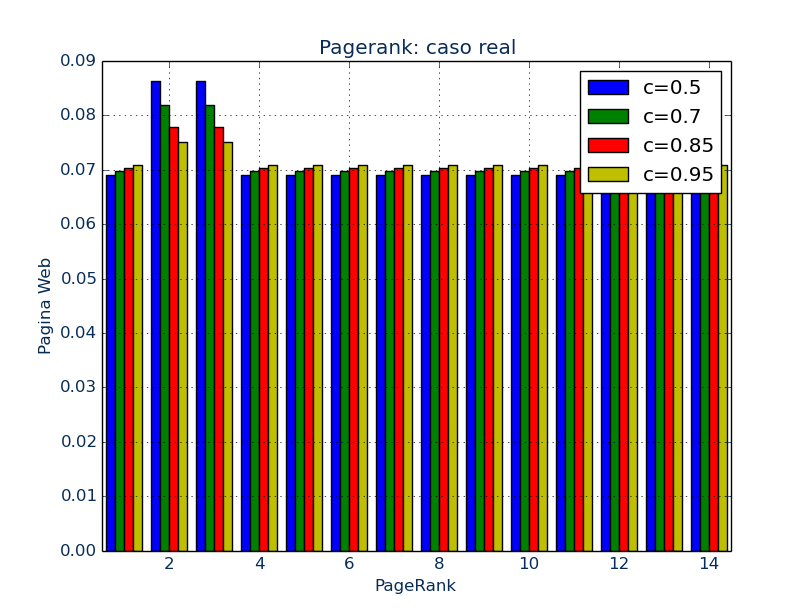
\includegraphics[scale=0.385]{img/PocosLinksout.png}
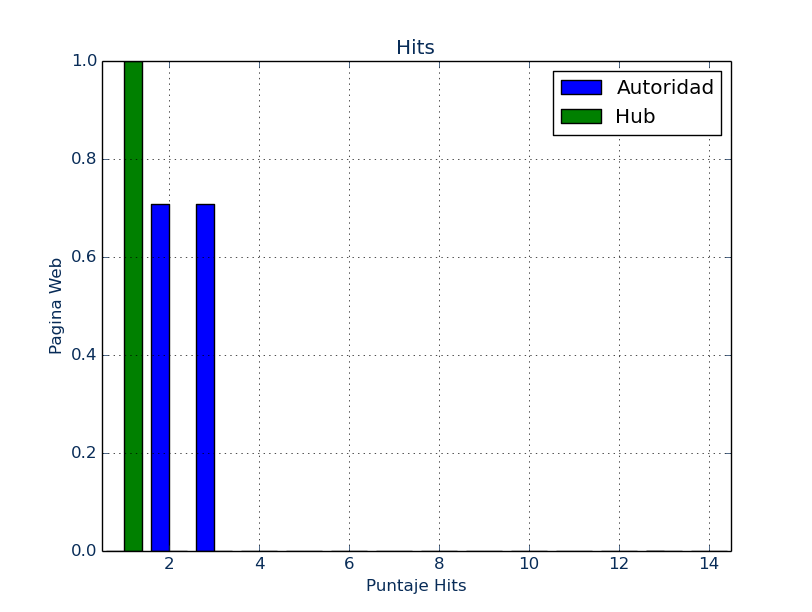
\includegraphics[scale=0.385]{img/PocosLinksoutH.png}
\caption{Puntajes obtenidos para una red con pocos links}
\end{figure}

\begin{figure}[htbp]
\centering
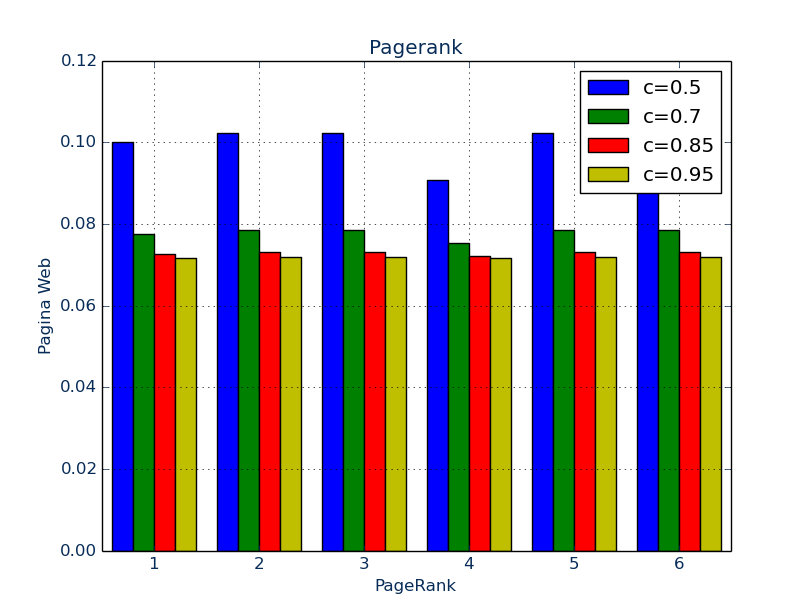
\includegraphics[scale=0.385]{img/muchoslinksout.png}
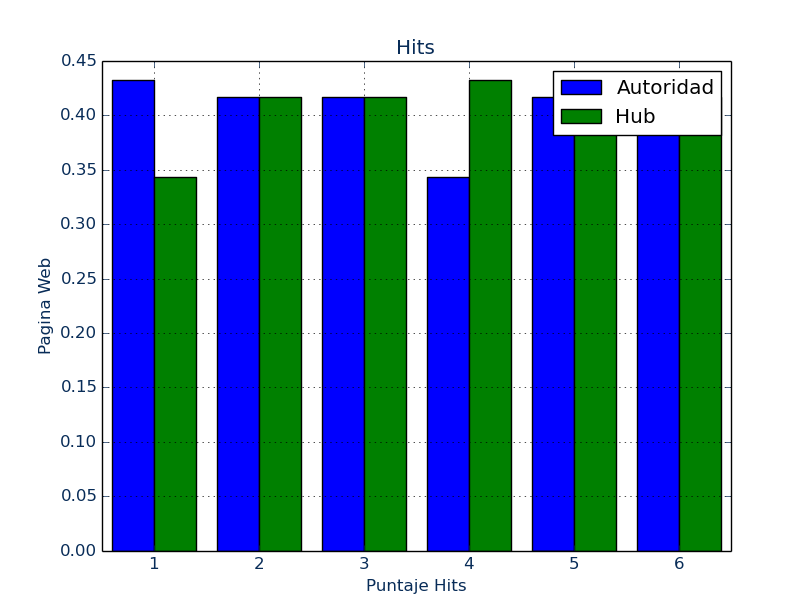
\includegraphics[scale=0.385]{img/muchoslinksoutH.png}
\caption{Puntajes obtenidos para una red con muchos links}
\end{figure}

\newpage
\section{Discusi\'{o}n}
\label{sec:discusion}
%Se incluirá aquí un análisis de los resultados obtenidos en la sección anterior (se analizará su validez, coherencia, etc.). Deben analizarse como mínimo los items pedidos en el enunciado. No es aceptable decir que “los resultados fueron los esperados”, sin hacer clara referencia a la teoría la cual se ajustan. Además, se deben mencionar los resultados interesantes y los casos “patológicos” encontrados.

En PageRank, las normas convergen a 0 en forma exponencial luego de las primeras iteraciones. Cuanto mayor sea el valor de $c$, más tarda en alcanzarse el criterio de parada. Como ya se dijo, en un caso extremo, con $c=1$, la norma podría no converger. En HITS, las normas también convergen a 0 en forma exponencial.\\

En todos los casos analizados se obtuvo que el tiempo de cómputo de PageRank aumentó exponencialmente con el valor de $c$.\\

El algoritmo HITS resultó más lento que PageRank para todos los valores de $c \leq 0,85$ que utilizamos, en todas las redes para las que medimos los tiempos. Sin embargo, consideramos que esta diferencia se debe principalmente a que el algoritmo HITS debe realizar dos productos entre una matriz y un vector, mientras que PageRank solo realiza una. Se puede comprobar que esta diferencia es proporcional al tamaño de la matriz que representa a la red. Es decir, la diferencia no llega a ser de órdenes de complejidad.\\

Además, se espera que si se eligen valores de $c$ mayores a un valor, el tiempo de ejecución de Pagerank siempre supere al de HITS.\\

En los tests de mayor tamaño se puede ver que la cantidad de iteraciones necesarias para alcanzar convergencia es igual que en los tests menores o incluso menor. Si tienen mayor tiempo de cómputo, es porque la multiplicación entre la matriz y el vector que es necesaria en cada iteración tiene una mayor cantidad de elementos. Esto se puede ver en el tiempo de iteración. Sin embargo, dada la proporción de links por páginas, esto tampoco influye demasiado.\\

El valor de $c$, si bien influye en el puntaje, no lo varía demasiado. Un valor más alto de $c$ implica darle una mayor importancia a los links que relacionan las páginas, resultando en un ranking más representativo de la estructura de la red. Sin embargo, no necesariamente será mejor como modelo para el comportamiento de un navegante aleatorio en la práctica.\\

Teniendo en cuenta que la cantidad de iteraciones, y por lo tanto el tiempo de ejecución, escalan exponencialmente con este parámetro, es conveniente elegir un valor no demasiado alto. \\

Al hacer un análisis cualitativo de los puntajes obtenidos se pueden obvervar que el puntaje no es el esperado. Por ejemplo, se esperaba que Google obtuviera el mayor puntaje de hub, cosa que no ocurrió.\\

Esto se debe a que la porción de la red elegida no es representativa. Se ve que lanacion.com obtuvo el mayor puntaje de PageRank, pero hay que tener en cuenta que en la lista hay sitios que pertenecen al mismo dominio.\\

\newpage

\section{Conclusiones}
\label{sec:conclusiones}

%Esta sección debe contener las conclusiones generales del trabajo. Se deben mencionar las relaciones de la discusión sobre las que se tiene certeza, junto con comentarios y observaciones generales aplicables a todo el proceso. Mencionar también posibles extensiones a los métodos, experimentos que hayan quedado pendientes, etc.

En el paper escrito por Brin y Page \footnote{Brin, Page - 1998 - The anatomy of a large-scale hypertextual Web search engine} se recomienda tomar un $c$ (probabilidad de un navegante aleatorio de seguir un link de la página en la que está) de 0.85.\\ \\%O sea, hacer experimentos 

Consideramos sin embargo que, de contar con los recursos necesarios para realizar mediciones de la magnitud necesaria para obtener resultados representativos, la mejor manera de definir un valor de $c$ fiable en la mayor cantidad de casos posibles sería acercarnos a la probabilidad real con la que el navegante aleatorio $salta$ a otra página sin seguir un link, para esto haría falta hacer experimentos con navegantes reales y realizar un promedio de los $c$ que obtuvimos de estos navegantes; es decir que el mejor $c$ a tomar sería la esperanza de los $c$ obtenidos en estas mediciones.\\

El hecho de que la norma converja exponencialmente permite que la cantidad de iteraciones sea lo suficientemente acotada, teniendo en cuenta que cada iteración es una multiplicación de una matriz por un vector que puede tener varios millones de posiciones.


Luego de haber contrastado estos distintos métodos de ranking podemos decir con seguridad que:\\


\textbf{In-Deg} es completamente descartable como método para decdidir la relevancia de una página, se limita a realizar el análisis más previsible y propenso a caer en errores.
Buscadores puramente textuales que siguieron este método, como AltaVista, fueron reemplazados eventualmente por otros más útiles, si bien fueron un paso necesario para la creación de buscadores mejores.\\\\

\textbf{HITS} es mucho más efectivo y confiable ya que realiza un análisis más inteligente de la red que le es proporcionada, confiriéndole distintos roles a las páginas y contrastándolas a partir de las relaciones entre estas páginas según el rol que estén cumpliendo.\\
Hemos comprobado que la cantidad de links a una página no son relevantes por sí solos para considerarla una buena autoridad sino que lo más importante es la relevancia como hubs de aquellas páginas que la apuntan, esto revela un análisis mucho más profundo que el de \textit{Indeg}.\\
Por la naturaleza del análisis que realiza es, sin embargo, más susceptible de caer en engaños tales como que páginas acuerden apuntarse entre sí para ganar peso en el ranking que \textit{HITS} les asigne, mientras que con \textit{PageRank} este artilugio no daría frutos debido a que cuantos más links salientes una página tenga, menos valor le estará transfiriendo con cada link a las páginas apuntadas.\\\\

\textbf{PageRank} es el método que consideramos mejor, superando tanto a \textit{HITS} como a \textit{Indeg} debido a que realiza un análisis profundo de las relaciones entre páginas, distinto de aquel proporcionado por \textit{HITS}. En ciertos casos parece que el procedimiento es opuesto. Por ejemplo, una página que apunta a todas le da poco valor a cada una en PageRank, pero al apuntar a muchas autoridades es un buen hub según HITS, luego le da valor a los que apunta. Un inconveniente que tiene este algoritmo es que trata una pagina con links a toda la web igual que un dangling node, mientras que HITS le da a un gran puntaje como hub.
\\\\

Por ultimo, si el cliente quiere tener un mejor PageRank, debe conseguir que lo apunten páginas que tengan la mejor proporción entre PageRank y cantidad de links salientes, ya que el puntaje se distribuye entre todas las páginas. En cambio, si quiere conseguir un mejor puntaje como autoridad en HITS, debe buscar que la mayor cantidad posible de las mejores páginas lo apunten. Si desea tener un mejor puntaje de hub tendría que apuntar a las páginas con mayor autoridad en HITS.\\
Podemos finalmente concluir que la mejor estrategia a sugerir a clientes sería darle prioridad al ranking proporcionado por Pagerank, está además la prueba de la efectividad del Pagerank en el éxito que tuvo Google al usarlo. 
Sugeriríamos entonces apoyarse en el orden de resultados que proporcione este buscador (que es además el más usado) para decidir en qué páginas comprar espacio de publicidad.

\newpage

\section{Apéndice A}
\label{sec:ApA}

\documentclass[11pt, a4paper]{article}
%\usepackage[spanish]{babel}
\usepackage{a4wide}
\usepackage{amsfonts}
\usepackage{graphicx}
\usepackage{verbatim}
\usepackage{todonotes}
\usepackage{amsmath}
\usepackage{url}

\usepackage{tikz}
\usetikzlibrary{decorations.markings,arrows}

\parindent = 0 pt
\parskip = 5 pt

\newcommand{\real}{\hbox{\bf R}}

\begin{document}
\begin{center}
\begin{tabular}{r|cr}
 \begin{tabular}{c}
{\large\bf\textsf{\ M\'etodos Num\'ericos\ }}\\ 
Segundo Cuatrimestre 2014\\
{\bf Trabajo Pr\'actico 2}\\
\end{tabular} &
\begin{tabular}{@{} p{1.6cm} @{}}

\includegraphics[width=1.6cm]{logodpt.jpg}
\end{tabular} &
\begin{tabular}{l @{}}
 \emph{Departamento de Computaci\'on} \\
 \emph{Facultad de Ciencias Exactas y Naturales} \\
 \emph{Universidad de Buenos Aires} \\
\end{tabular} 
\end{tabular}
\vskip 10pt
\textbf{\Large Tirate un qu\'e, tirate un \emph{ranking}...}
\end{center}

\vskip 10pt
\hrule
\vskip 5pt

\noindent\textbf{Motivaci\'on}
\vskip 5pt

Luego de su repentina y ef\'imera irrupci\'on durante el a\~no 2011, un grupo de la movida tropical\footnote{Por
cuestiones de privacidad, no haremos p\'ublico de qu\'e grupo se trata.} est\'a buscando recuperar la notoriedad y los niveles 
de popularidad otrora alcanzados. El retorno incluye, entre otras cosas, un mega recital gratuito, giras por las
principales \emph{bailantas} y por el interior del pa\'is.\footnote{A riesgo de exponer su edad, los miembros de la c\'atedra 
quieren destacar a aquellos pr\'oceres que llevaron a este g\'enero musical a las primeras planas, como Alcides, Sebasti\'an, 
Miguel \emph{Conejito} Alejandro, R\'afaga, La Nueva Luna, Comanche y, como dejar fuera, al \emph{MAESTRO} Antonio R\'ios.}

Para que toda esta movida sea exitosa, los miembros del grupo han acordado con su \emph{community manager} que, adem\'as de
tener una participaci\'on destacada en Pasi\'on de S\'abado, es necesario que la llegada a trav\'es de los medios electr\'onicos
y las redes sociales sea muy efectiva, al igual que en 2011, alcanzando a la mayor cantidad posible de gente y poder, nuevamente, 
sentarse en el living de \emph{la diva de los tel\'efonos}. La conclusi\'on a la que llegaron es que necesitan que cada vez que 
realiza una b\'usqueda relacionada con la movida tropical, su p\'agina se encuentre entre las primeras que muestran los buscadores.

Con ese motivo, se han contactado con el equipo de R+D de M\'etodos Num\'ericos, donde en la primera reuni\'on el cliente propuso
\emph{comprar clicks en publicidades}. Esta, si bien es una alternativa viable, representa un gasto importante para la escala de
inversi\'on con la que se dispone. Luego de una reuni\'on del equipo t\'ecnico, se les hizo una contrapropuesta:
estudiar el comportamiento de los buscadores y, a cambio de shows libres de costo y presentaciones privadas, buscar en qu\'e
p\'aginas conviene figurar para mejorar el posicionamiento virtual del grupo.
 
\vskip 5pt
\noindent\textbf{Contexto}
\vskip 5pt

A partir de la evoluci\'on de Internet durante la d\'ecada de 1990, el desarrollo de motores de b\'usqueda se ha convertido
en uno de los aspectos centrales para su efectiva utilizaci\'on. Hoy en d\'ia, sitios como Yahoo, Google y Bing ofrecen
distintas alternativas para realizar b\'usquedas complejas dentro de un red que contiene miles de millones de p\'aginas
web. 

En sus comienzos, una de las caracter\'isticas que distngui\'o a Google respecto de los motores de b\'usqueda de la \'epoca
fue la calidad de los resultados obtenidos, mostrando al usuario p\'aginas relevantes a la
b\'usqueda realizada. El esquema general de los or\'igenes de este motor de b\'usqueda es brevemente explicando en 
Brin y Page \cite{Brin1998}, donde se mencionan aspectos t\'ecnicos que van desde la etapa de obtenci\'on de
informaci\'on de las p\'aginas disponibles en la red, su almacenamiento e indexado y su posterior procesamiento,
buscando ordenar cada p\'agina de acuerdo a su importancia relativa dentro de la red. El algoritmo utilizado para esta
\'ultima etapa es denominado PageRank y es uno (no el \'unico) de los criterios utilizados para ponderar la importancia
de los resultados de una b\'usqueda. En este trabajo nos concentraremos en el estudio y desarrollo del algoritmo
PageRank.

\vskip 5pt
\noindent\textbf{Los m\'etodos, Parte I: PageRank}
\vskip 5pt

El algoritmo PageRank se basa en la construcci\'on del siguiente modelo. Supongamos que tenemos una red con $n$ p\'aginas 
web $Web = \{1,\dots,n\}$ donde
el objetivo es asignar a cada una de ellas un puntaje que determine la importancia relativa de la misma respecto de las
dem\'as. Para modelar las relaciones entre ellas, definimos la \emph{matriz de conectividad} $W \in \{0,1\}^{n \times n}$ 
de forma tal que $w_{ij} = 1$ si la p\'agina $j$ tiene un link a la p\'agina $i$, y $w_{ij} = 0$ en caso contrario. 
Adem\'as, ignoramos los \emph{autolinks}, es decir, links de una p\'agina a s\'i misma, definiendo $w_{ii} = 0$. Tomando 
esta matriz, definimos el grado de la p\'agina $j$, $n_j$, como la cantidad de links salientes hacia otras p\'aginas 
de la red, donde $n_j = \sum_{i = 1}^n w_{ij}$. Adem\'as, notamos con $x_j$ al puntaje asignado a la p\'agina $j\in
Web$, que es lo que buscamos calcular.

La importancia de una p\'agina puede ser modelada de diferentes formas. Un link de la p\'agina $u \in
Web$ a la p\'agina $v \in Web$ puede ser visto como que $v$ es una p\'agina importante. Sin embargo, no queremos que una
p\'agina obtenga mayor importancia simplemente porque es apuntada desde muchas p\'aginas. 
Una forma de limitar esto es ponderar los links utilizando la importancia de la p\'agina de origen. En otras palabras,
pocos links de p\'aginas importantes pueden valer m\'as que muchos links de p\'aginas poco importantes. En particular,
consideramos que la importancia de la p\'agina $v$ obtenida mediante el link de la p\'agina $u$ es proporcional a la 
importancia de la p\'agina $u$ e inversamente proporcional al grado de $u$. Si la p\'agina $u$ contiene $n_u$ links,
uno de los cuales apunta a la p\'agina $v$, entonces el aporte de ese link a la p\'agina $v$ ser\'a $x_u/n_u$. Luego,
sea $L_k \subseteq Web$ el conjunto de p\'aginas que tienen un link a la p\'agina $k$. Para cada p\'agina pedimos que
\begin{eqnarray}
x_k = \sum_{j \in L_k} \frac{x_j}{n_j},~~~~k = 1,\dots,n. \label{eq:basicmodel}
\end{eqnarray}
Definimos $P \in  \mathbb{R}^{n \times n}$ tal que $p_{ij} = 1/n_j$ si $w_{ij} = 1$, y $p_{ij} = 0$ en caso contrario. Luego,
el modelo planteado en (\ref{eq:basicmodel}) es equivalente a encontrar un $x\in \mathbb{R}^n$ tal que $Px = x$, es
decir, encontrar (suponiendo que existe) un autovector asociado al autovalor 1 de una matriz cuadrada, tal que $x_i \ge
0$ y $\sum_{i = 1}^n x_i = 1$. En
Bryan y Leise \cite{Bryan2006} y Kamvar et al. \cite[Secci\'on 1]{Kamvar2003} se analizan ciertas condiciones que debe
cumplir la red de p\'aginas para garantizar la existencia de este autovector.

Una interpretaci\'on equivalente para el problema es considerar al \emph{navegante aleatorio}. \'Este empieza en una
p\'agina cualquiera del conjunto, y luego en cada p\'agina $j$ que visita sigue navegando a trav\'es de sus links,
eligiendo el mismo con probabilidad $1/n_j$. Una situaci\'on particular se da cuando la p\'agina no tiene links salientes. En
ese caso, consideramos que el navegante aleatorio pasa a cualquiera de las p\'agina de la red con probabilidad $1/n$.
Para representar esta situaci\'on, definimos $v \in \mathbb{R}^{n \times n}$, con $v_i = 1/n$ y $d \in \{0,1\}^{n}$ donde 
$d_i = 1$ si $n_i = 0$, y $d_i = 0$ en caso contrario. La nueva matriz de transici\'on es 
\begin{eqnarray*}
D & = & v d^t \\
P_1 & = & P + D.
\end{eqnarray*}
Adem\'as, consideraremos el caso de que el navegante aleatorio, dado que se encuentra en la p\'agina $j$, decida visitar
una p\'agina cualquiera del conjunto, independientemente de si esta se encuentra o no referenciada por $j$ (fen\'omeno
conocido como \emph{teletransportaci\'on}). Para ello, consideramos que esta decisi\'on se toma con una probabilidad
$c \ge 0$, y podemos incluirlo al modelo de la siguiente forma:
\begin{eqnarray*}
E & = & v \bar{1}^t \\
P_2 & = & cP_1 + (1-c)E,
\end{eqnarray*}
\noindent donde $\bar{1} \in \mathbb{R}^n$ es un vector tal que todas sus componenetes valen 1. La matriz resultante
$P_2$ corresponde a un enriquecimiento del modelo formulado en (\ref{eq:basicmodel}). Probabil\'isticamente, la
componente $x_j$ del vector soluci\'on (normalizado) del sistema $P_2 x = x$ representa la proporci\'on del tiempo que,
en el largo plazo, el navegante aleatorio pasa en la p\'agina $j \in Web$.

En particular, $P_2$ corresponde a una
matriz \emph{estoc\'astica por columnas} que cumple las hip\'otesis planteadas en Bryan y Leise \cite{Bryan2006} y
Kamvar et al. \cite{Kamvar2003}, tal que $P_2$ tiene un autovector asociado al autovalor 1, los dem\'as autovalores de
la matriz cumplen $1 = \lambda_1 > |\lambda_2| \ge \dots \ge |\lambda_n|$ y, adem\'as, la dimensi\'on
del autoespacio asociado al autovalor $\lambda_1$ es 1. Luego, la soluci\'on al sistema $P_2 x = x$ puede ser calculada
de forma est\'andar utilizando el m\'etodo de la potencia.

Una vez calculado el ranking, se retorna al usuario las $t$ p\'aginas con mayor ranking.

\vskip 5pt
\noindent\textbf{Los m\'etodos, Parte II: Hyperlink-Induced Topic Search}
\vskip 5pt

Un m\'etodo alternativo es propuesto en Kleinberg \cite{Kleinberg}, denominado \emph{Hyperlink-Induced Topic Search} (HITS). La 
intuici\'on del m\'etodo se basa en el an\'alisis intr\'iniseco de la red, donde una noci\'on de \emph{autoridad} se 
transfiere de una p\'agina a otra mediante los links que las relacionan. El objetivo es, dada una b\'usqueda concreta,
retornar un subconjunto acotado de p\'aginas relevantes. Con este fin, se considera que existen p\'aginas que cumplen un 
rol de \emph{autoridad} sobre un tema espec\'ifico y se busca modelar la relaci\'on entre estas p\'aginas y aquellas que 
apuntan a varias de estas autoridades, denominadas \emph{hubs}. En la pr\'actica, los autores observan que suele existir
una especie de equilibrio en la relaci\'on entre hubs y autoridades, y se busca aprovechar esta relaci\'on para el desarrollo
del algoritmo. Intuitivamente, un buen \emph{hub} es una p\'agina que apunta a muchas autoridades, y una buena \emph{autoridad}
es una p\'agina que es apuntada por muchos \emph{hubs}.

El procedimiento consiste en los siguientes pasos. Dada una b\'usqueda concreta, se utiliza en primer lugar un \emph{buscador}
simple (por ejemplo, basado en texto) para obtener un conjunto acotado de paginas (digamos, 200), llamado \emph{root set}. 
Luego, asumiendo que la estructura de la red es conocida, es busca extender este conjunto agregando p\'aginas que son apuntadas
y que apuntan a las p\'aginas de \emph{root set}, hasta llegar a una sub-red de un tama\~no determinado. En el contexto del
trabajo pr\'actico, asumiremos que este paso ha sido realizado y que contamos con el grafo que considera la sub-red.

Formalmente, y retomando la notaci\'on introducida en la secci\'on anterior, consideramos que las p\'aginas de nuestra sub-red
se encuentran en el conjunto $Web = \{1,\dots,n\}$. Para modelar las relaciones entre las p\'aginas, adoptamos una definici\'on 
similar: consideramos la matriz de adyacencia $A \in \{0,1\}^{n \times n}$ donde $a_{ij} = 1$ si existe un link de la p\'agina
$i$ a la p\'agina $j$.\footnote{Notar que $A = W^t$.} Para cada p\'agina $i \in Web$ se considera el \emph{peso de autoridad} $x_i$ 
y el \emph{peso de hub} $y_i$. Consecuentemente, se definen los vectores $x,y \in \mathbb{R}^n$ los vectores de pesos de autoridad
y hubs, respectivamente, y supondremos adem\'as que se encuentran normalizados. Las p\'aginas con mayores valores de $x_i$ e $y_i$
son consideradas mejores \emph{autoridades} y \emph{hubs}, respectivamente.

La relaci\'on mencionada entre los distintos tipos de p\'aginas se expresan num\'ericamente de la siguiente forma. Dados los
vectores $x,y$, la operaci\'on de transferencia de los \emph{hubs} a la autoridad $j \in Web$ puede expresarse de la siguiente forma:
\begin{equation}
x_j = \sum_{i: i \to j} y_i. \label{eq:auth-update}
\end{equation}
An\'alogamente, el peso de un hub est\'a dado por la siguiente ecuaci\'on
\begin{equation}
y_i = \sum_{j: i \to j} x_j. \label{eq:hub-update}
\end{equation}

Las ecuaciones (\ref{eq:auth-update}) y (\ref{eq:hub-update}) podemos expresarlas matricialmente de la siguiente manera:
\begin{eqnarray}
x & = & A^ty \label{eq:auth-update-math} \\
y & = & Ax, \label{eq:hub-update-math} 
\end{eqnarray}
aplicando luego el paso de normalizaci\'on correspondiente. Los autores proponen comenzar con un $y_0$ incial, aplicar estas ecuaciones 
iterativamente y demuestran que, bajo ciertas condiciones, el m\'etodo converge. Finalmente, en base a los rankings obtenimos, se retorna
al usuario las mejores $t$ \emph{autoridades} y los mejores $t$ \emph{hubs}.

\vskip 5pt
\noindent\textbf{Enunciado}
\vskip 5pt

El objetivo del trabajo es experimentar en el contexto planteado utilizando los algoritmos de ranking propuestos. Para ello, se considera
un entorno que, dentro de nuestras posibilidades, simule el contexto real de aplicaci\'on donde se abordan instancias de gran escala (es
decir, $n$, el n\'umero total de p\'aginas, es grande). El archivo tomar\'a como entrada un archivo que especifique el algoritmo, los
par\'ametros del mismo y un puntero al grafo de la red y retorne como resultado el ranking obtenido para cada p\'agina. Los detalles sobre 
el input/output del programa son especificados en la siguiente secci\'on.

El trabajo consistir\'a en estudiar distintos aspectos de los siguientes m\'etodos: PageRank, HITS, e \textsc{In-deg}, \'este \'ultimo consiste
en definir el ranking de las p\'aginas utilizando solamente la cantidad de ejes entrantes a cada una de ellas, orden\'andolos en forma
decreciente. Para tener una descripci\'on m\'as completa de los dos primeros m\'etodos, se propone:
\begin{enumerate}
\item Considerar el trabajo de Kleinberg \cite{Kleinberg} con los detalles sobre HITS, en particular las secciones 1, 2 y 3.
\item Considerar el trabajo de Bryan y Leise \cite{Bryan2006} donde se explica la intuci\'on y algunos detalles t\'ecnicos respecto a PageRank. Adem\'as, 
en Kamvar et al. \cite{Kamvar2003} se propone una mejora del mismo. Si bien esta mejora queda fuera de los alcances del trabajo, en la Secci\'on 1 se
presenta una buena formulaci\'on del algoritmo. En base a su definici\'on, $P_2$ no es una matriz esparsa. Sin embargo, en Kamvar et al. 
\cite[Algoritmo 1]{Kamvar2003} se propone una forma alternativa para computar $x^{(k+1)} = P_2 x^{(k)}$. Este resultado puede ser utilizado
para mejorar el almacenamiento de los datos.
\item (Opcional) Completar la demostraci\'on del Teorema 3.1 de Kleinberg \cite{Kleinberg}, incluyendo el detalle de los puntos que el autor asume como 
triviales.
\end{enumerate}

En la pr\'actica, el grafo que representa la red de p\'aginas suele ser esparso, es decir, una p\'agina posee relativamente pocos links
de salida comparada con el n\'umero total de p\'aginas. A su vez, dado que $n$ tiende a ser un n\'umero muy grande, es importante tener
en cuenta este hecho a la hora de definir las estructuras de datos a utilizar. Luego, desde el punto de vista de implementaci\'on se pide
utilizar alguna de las siguientes estructuras de datos para la representaci\'on de las matrices esparsas: \emph{Dictionary of Keys} (dok), 
\emph{Compressed Sparse Row} (CSR) o \emph{Compressed Sparse Column} (CSC). Se deber\'a incluir una justificaci\'on respecto a la elecci\'on 
que consdiere el contexto de aplicaci\'on. Una vez definida la estructura a utilizar, se deber\'a implementar el algoritmo HITS utilizando
las ecuaciones (\ref{eq:auth-update-math}) y (\ref{eq:hub-update-math}). Para el caso de PageRank, se debe implementar el m\'etodo de la
potencia para calcular el autovector principal.

En funci\'on de la experimentaci\'on, se deber\'a realizar un estudio particular para cada algoritmo (tanto en t\'erminos de comportamiento
del mismo, como una evaluaci\'on de los resultados obtenidos) y luego se proceder\'a a comparar cualitativamente los rankings generados.
La experimentaci\'on deber\'a incluir como m\'inimo los siguientes experimentos:
\begin{enumerate}
\item Estudiar la convergencia de PageRank, analizando la evoluci\'on de la norma Manhattan (norma $L_1$) entre dos iteraciones sucesivas. Comparar
los resultados obtenidos para al menos dos instancias de tama\~no mediano-grande, variando el valor de $c$. Opcional: Establecer una relaci\'on 
con la proporci\'on entre $\lambda_1 = 1$ y $|\lambda_2|$.
\item Estudiar la convergencia de los vectores de peso $x$ e $y$ para HITS de forma similar al punto anterior.
\item Estudiar el tiempo de c\'omputo requerido por PageRank y HITS. Si bien ambos pueden se aplicados sobre una red gen\'erica, cada algoritmo 
tiene un contexto particular de aplicaci\'on. Estudiar como impacta el factor temporal en este sentido.
\item Estudiar cualitativamente los rankings obtenidos por los tres m\'etodos. Para ello, se sugiere considerar distintos ejemplos de b\'uquedas
de p\'aginas web\footnote{La c\'atedra adjunta casos de \emph{benchmark} que representan sub-redes obtenidas en base a b\'usquedas tem\'aticas}.
Analizar los resultados individualmente en una primera etapa, y luego realizar un an\'alisis comparativo entre los tres rankings obtenidos.
\item Para cada algoritmo, proponer ejemplos de tama\~no peque\~no que ilustren el comportamiento esperado (puede ser utilizando las instancias
provistas por la c\'atedra o generadas por el grupo).
\end{enumerate}

Finalmente, y en base a la experimentaci\'on realizada, buscamos resolver el problema planteado originalmente: dada una foto de la red, con sus
interconexiones entre p\'aginas, supongamos que tenemos los pesos (ranking) asignados por uno de los algoritmos estudiados. ?`Cu\'al ser\'ia la
estrategia que le sugiere al cliente para mejorar su correspondiente ranking? Para este \'ultimo punto, suponer que es posible \emph{negociar}
que una p\'agina apunte a nuestro sitio, y que la cantidad de estas negociaciones que podemos tener es acotada.

\vskip 5pt
\noindent\textbf{Par\'ametros y formato de archivos}
\vskip 5pt

El programa deber\'a tomar por l\'inea de comandos dos par\'ametros. El primero de ellos contendr\'a la informaci\'on del experimento, incluyendo
el m\'etodo a ejecutar (\verb+alg+, 0 para PageRank, 1 para HITS, 2 para \textsc{In-deg}), la probabilidad de teletransportaci\'on $c$ en el caso
de PageRank (que valdr\'a -1 si \verb+alg+ no es 0), el tipo de instancia, el \emph{path} al archivo/directorio conteniendo la definici\'on de la red (que debe ser relativa
al ejecutable, o el path absoluto al archivo) y el valor de 
tolerancia utilizado en el criterio de parada impuesto a cada m\'etodo. El siguiente ejemplo muestra un caso donde se pide ejecutar PageRank, con una
probabilidad de teletransportaci\'on de 0.85, sobre la red descripta en \verb+red-1.txt+ (que se encuentra en el directorio \verb+tests/+) y con una 
tolerancia de corte de $0.0001$.
\begin{verbatim}
0 0.85 0 tests/red-1.txt 0.0001
\end{verbatim}

Para la definici\'on del grafo que representa la red, se consideran dos bases de datos de instancias con sus correspondientes formatos. La primera
de ellas es el conjunto provisto en SNAP \cite{SNAP} (el tipo de instancia es 0), con redes de tama\~no grande obtenidos a partir de datos reales. Adem\'as, se consideran las 
instancias propuestas en \cite{dataset}. Estas instancias son de tama\~no mediano, obtenidas tambi\'en en base a datos reales, y corresponden a redes
tem\'aticas obtenidas a partir de una b\'usqueda particular. Para cada nodo de la red se tiene: la direccion URL, una breve descripci\'on, y las 
p\'aginas a las cuales apunta. Si bien algunas de las URL ya no son v\'alidas, la descripci\'on permite tener algo m\'as de informaci\'on para 
realizar un an\'alisis cualitativo.

En el caso de la base de SNAP, los archivos contiene primero cuatro l\'ineas con informaci\'on sobre la instancia (entre ellas, $n$ y la cantidad
total de links, $m$) y luego $m$ l\'ineas con los pares $i$, $j$ indicando que $i$ apunta a $j$. A modo de ejemplo, a continuaci\'on se muestra el 
archivo de entrada correspondiente a la red propuesta en Bryan y Leise \cite[Figura 1]{Bryan2006}: 

\begin{verbatim}
# Directed graph (each unordered pair of nodes is saved once): 
# Example shown in Bryan and Leise.
# Nodes: 4 Edges: 8 
# FromNodeId    ToNodeId
1   2
1   3
1   4
2   3
2   4
3   1
4   1
4   3
\end{verbatim}

Para la otras instancias, en \cite{dataset} puede encontrarse una descripci\'on del formato propuesto (el tipo de instancia ser\'a 1 en este caso).

Una vez ejecutado el algoritmo, el programa deber\'a generar un archivo de salida que contenga una l\'inea por cada
p\'agina ($n$ l\'ineas en total), acompa\~nada del puntaje obtenido por el algoritmo PageRank/\textsc{In-deg}. En el caso de HITS, el archivo 
contendr\'a $2n$ l\'ineas, las primeras $n$ con el \emph{peso de autoridad} y las segundas $n$ con el \emph{peso de hub} para los v\'ertices
$1,\dots.n$.

Para generar instancias, es posible utilizar el c\'odigo Python provisto por la c\'atedra. La utilizaci\'on del mismo se
encuentra descripta en el archivo README. Es importante mencionar que, para que el mismo funcione, es
necesario tener acceso a Internet. En caso de encontrar un bug en el mismo, por favor contactar a los docentes de la
materia a trav\'es de la lista. Desde ya, el c\'odigo puede ser modificado por los respectivos grupos agregando todas
aquellas funcionalidades que consideren necesarias.

\vskip 5pt

\hrule

\vskip 5pt


{\bf \underline{Fechas de entrega}}
\begin{itemize}
 \item \emph{Formato Electr\'onico:} S\'abado 11 de Octubre de 2014, hasta las 23:59 hs, enviando el trabajo (informe +
 c\'odigo) a la direcci\'on \verb+metnum.lab@gmail.com+. El subject del email debe comenzar con el texto \verb+[TP2]+
 seguido de la lista de apellidos  de los integrantes del grupo.
 \item \emph{Formato f\'isico:} Mi\'ercoles 15 de Octubre de 2014, a las 17 hs. en la clase te\'orica.
\end{itemize}

\noindent \textbf{Importante:} El horario es estricto. Los correos recibidos despu\'es de la hora indicada ser\'an considerados re-entrega.  

\bibliographystyle{plain}
\bibliography{tp2}
\end{document}



\newpage
%En el apéndice B se incluirán los códigos fuente de las funciones relevantes desde el punto de vista numérico. Resultados que valga la pena mencionar en el trabajo pero que sean demasiado específicos para aparecer en el cuerpo principal del trabajo podrán mencionarse en sucesivos apéndicesaerotulados con las letras mayúsculas del alfabeto romano. Por ejemplo: [la demostración de una propiedad que aplican para optimizar el algoritmo que programaron para resolver un problema].

\section{Referencias}
\label{sec:ref}

Apuntes de clase

R. Burden y J.D.Faires, Análisis numérico, International Thomson Editors, 1998

http://www.cs.toronto.edu/~tsap/experiments/datasets/.

Stanford large network dataset collection. http://snap.stanford.edu/data/#web.

Sergey Brin and Lawrence Page. The anatomy of a large-scale hypertextual Web search engine. Computer Networks and ISDN Systems, 30(1-7):107–117, April 1998.

Kurt Bryan and Tanya Leise. The linear algebra behind google. SIAM Review, 48(3):569–581, 2006.

Sepandar D. Kamvar, Taher H. Haveliwala, Christopher D. Manning, and Gene H. Golub. Extrapolation methods for accelerating pagerank computations. In Proceedings of the 12th international conference on World Wide Web, WWW ’03, pages 261–270, New York, NY, USA, 2003. ACM.

Jon M. Kleinberg. Authoritative sources in a hyperlinked environment. 46(5):604–632, September 1999.


\end{document}